\documentclass[aspectratio=169]{beamer}

\usepackage[numbers,sort&compress]{natbib}
\usetheme {default}

\setbeamertemplate{footline}{
  \hfill
  \normalsize\insertframenumber
  \kern1em\vskip2pt
}
\setbeamertemplate{navigation symbols}{}

% Title page details
\title{Deconstructing Retrieval Abilities of Language Models}
\author{Hauke Tristan Hinrichs}
\institute{Faculty of Electrical Engineering and Computer Science \\
Institute of Data Science \\
Department of Knowledge-based Systems \\
L3S Research Center}
\date{\today}
\titlegraphic{
    \makebox[0.9\textwidth]{
        
\includegraphics[width=3.2cm,keepaspectratio]{figures/logo_luh.png}%
        \hfill
        
\includegraphics[width=2cm,keepaspectratio]{figures/LS3-logo-WEB (1).png}%
    }
}
        
\begin{document}

% TODO: 
% - Backup frame about tct colbert

\begin{frame}
    \titlepage
\end{frame}

% \begin{frame}{Outline}
%     \begin{enumerate}
%         \item Motivation
%         \item Research Questions
%         \item Approach
%         \item Results
%         \item Conclusion
%     \end{enumerate}
% \end{frame}

\begin{frame}{Motivation}
    \begin{itemize}
        \item Information Retrieval (IR) decides which information is presented to us
    \end{itemize}
    \begin{figure}[!ht]
        \centering
        \makebox[\textwidth][c]{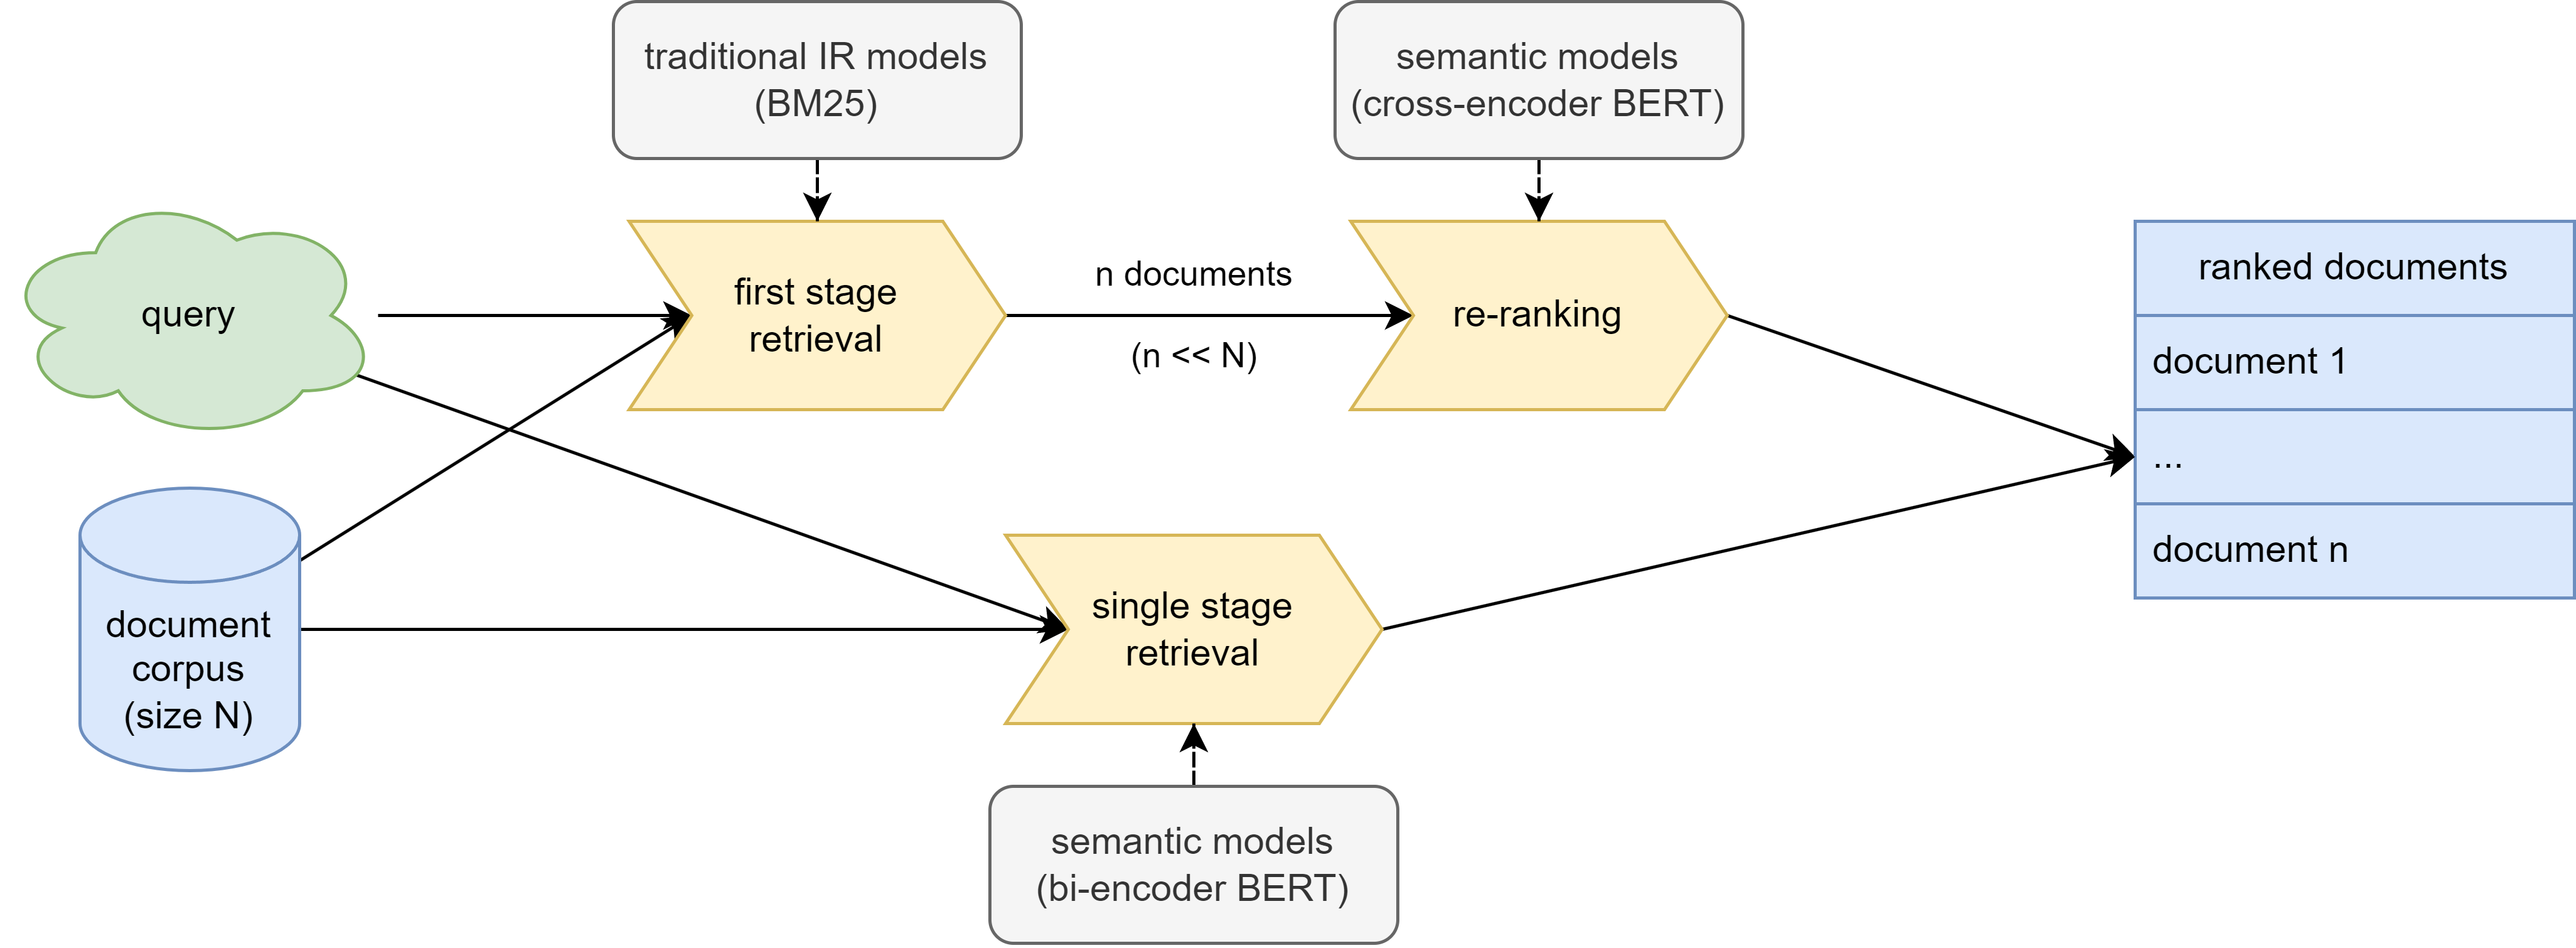
\includegraphics[width=0.9\textwidth]{figures/ir_overview.drawio.png}}
    \end{figure}
    \cite{bm25,Robertson1994OkapiAT,Bert_and_Beyond}
    \begin{itemize}
        \item Goal: shed light on inner workings of bi-encoder TCT-ColBERT \cite{tct_colbert,tct_colbert2}
    \end{itemize}
\end{frame}
% IR: (searching documents in corpus, query conveys information need) 
% IR decides what we get to see; large corpora (web) call for IR models (otherwise information not retrievable -> lost)
% Traditional: Exact-term matching and corpus statistics (IDF); highly performant (BoW)
% Neural models: possibility of semantic matching, but only performant in re-ranking
% Bi-encoder: first-stage or single-stage retrieval
% Goal: shed light how these models perform IR

\begin{frame}{Motivation -- Probing}
    \begin{itemize}
        \item Probing: technique to \textit{probe} for encoded information in the representations of language models (LMs) \cite{Tenney__Probing_for_Sentence_Structure_in_Contextualized_Word_Representations,Conneau__What_you_can_cram_into_a_single_vector,Adi__Fine-grained_Analysis_of_Sentence_Embeddings_Using_Auxilliary_Prediction}
    \end{itemize}
    \begin{figure}[!ht]
        \centering
        \makebox[\textwidth][c]{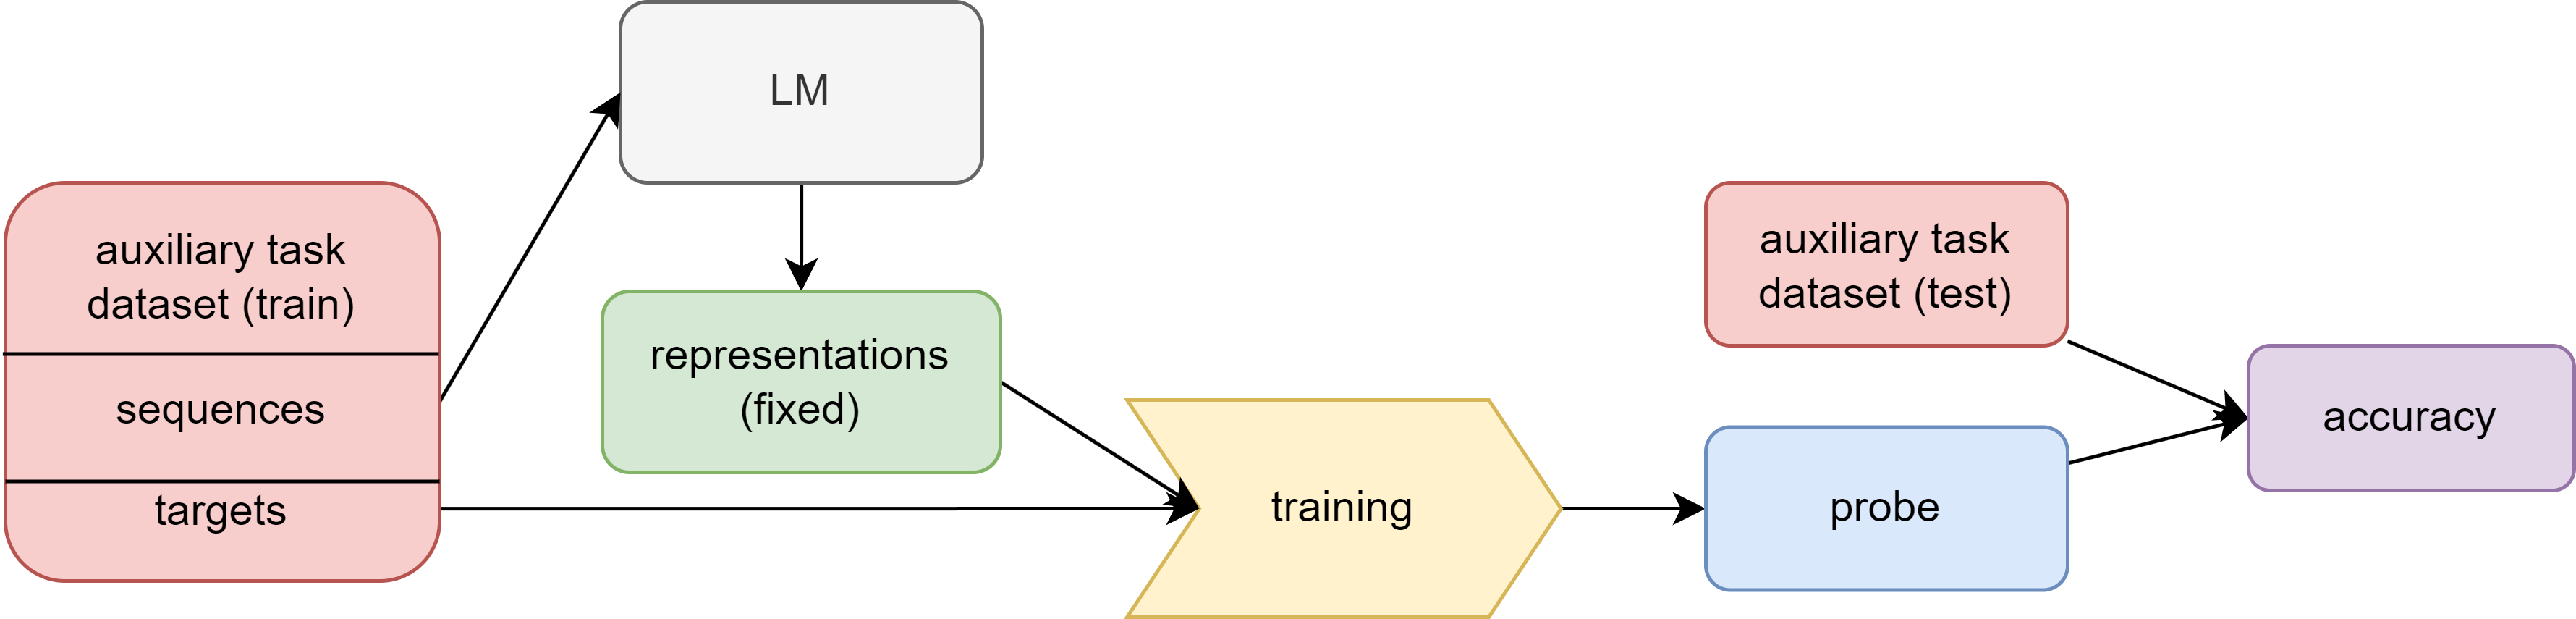
\includegraphics[width=0.7\textwidth]{figures/probing_overview (2).png}}
    \end{figure}
    \begin{itemize}
        \item Problem: encoding of information no proof for usage \cite{Ravichander__Probing_the_Probing_Paradigm}
        \item \textit{Causal Probing}: enabling causal explanations for model behavior by extending probing \cite{Elazar__Amnesic_Probing}
    \end{itemize}
\end{frame}
% Probing: technique to measure if information about properties encoded
% Small classifier trained on fixed representations to predict a property of interest
% Problem encoding no proof for usage: encoding can happen through pre-training (might be irrelevant for downstream task) or even accidentally
% Solution: Counterfactual White-Box Approach: Linear probe trained for task -> property removal projection

\begin{frame}{Research Questions}
    \begin{itemize}
        \item \textbf{RQ1} Can we confirm the feasibility of \textit{causally probing} our bi-encoder subject model in the context of retrieval?
        \item \textbf{RQ2} On which properties does our bi-encoder rely upon to solve the task of text retrieval?
        \item \textbf{RQ3} At which layers are important properties encoded?
    \end{itemize}
\end{frame}
% Feasibility studies: Investigate removal technique confirm feasibility of our approach (extension of probing!)
% RQ2 next slide covers investigated properties
% RQ3 not only encoded but also used

\begin{frame}{Approach -- Causal Probing: Key Idea}
    \begin{figure}[!ht]
        \centering
        \makebox[\textwidth][c]{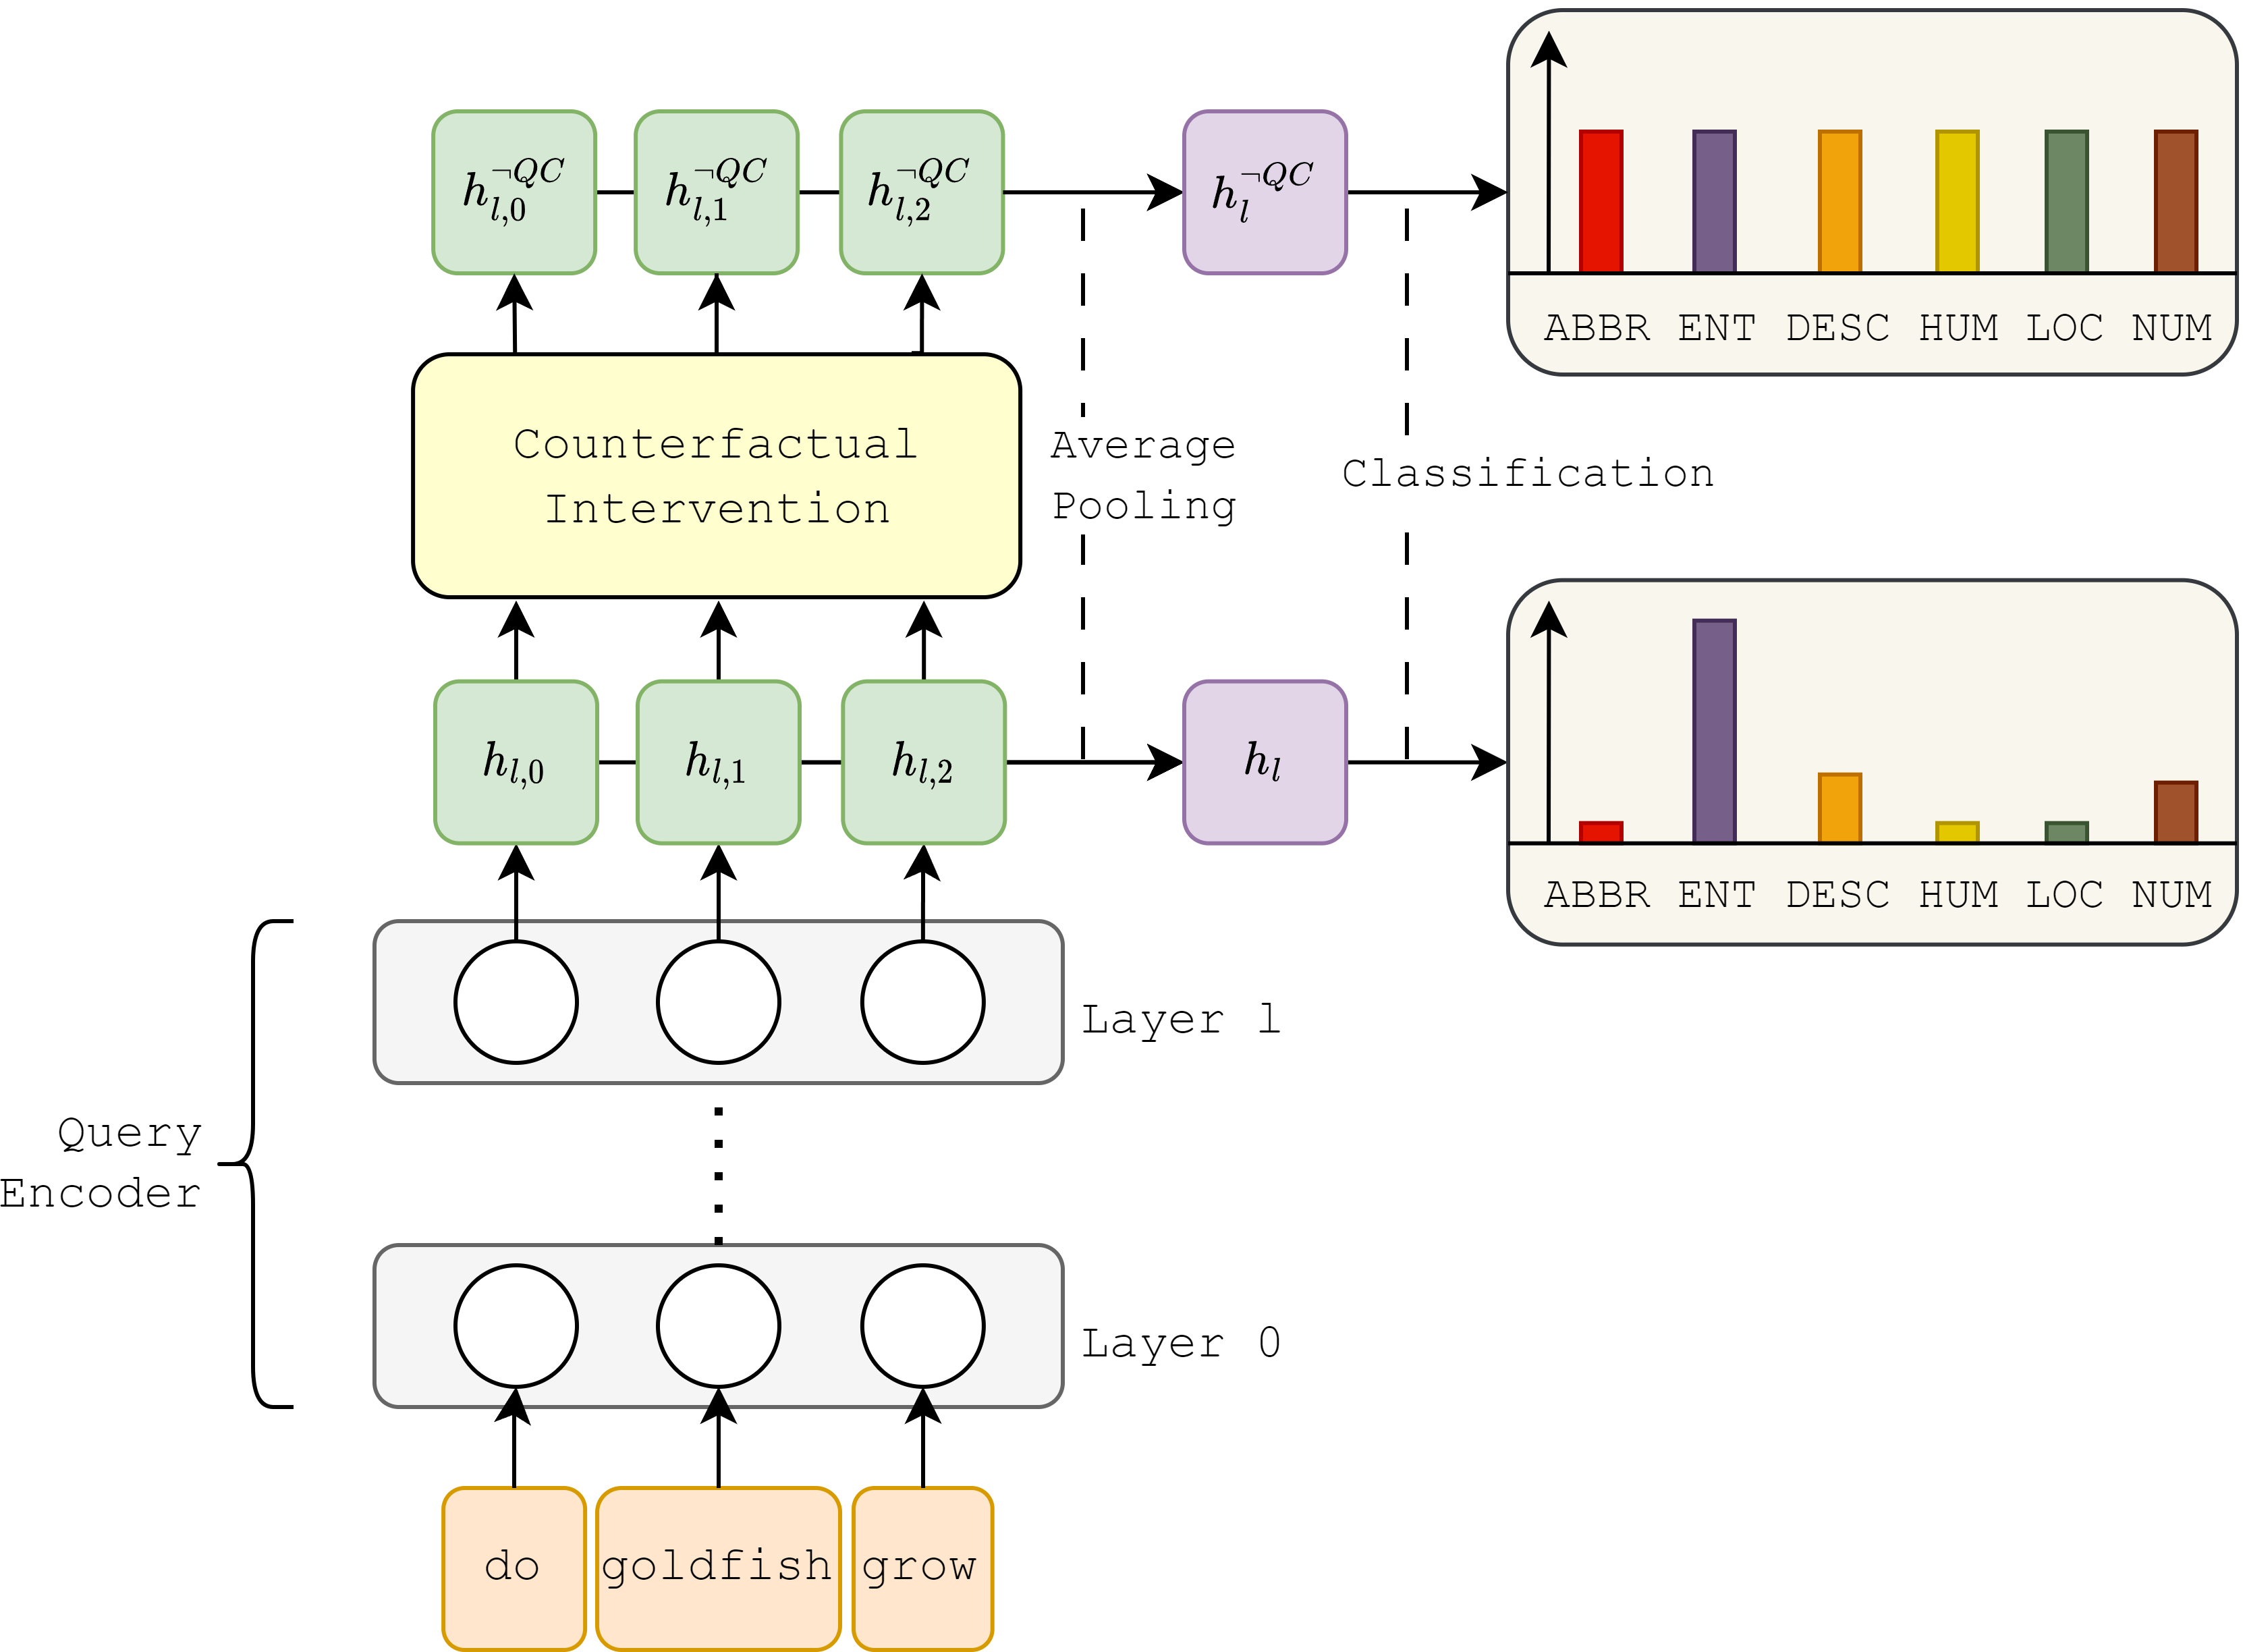
\includegraphics[width=0.75\textwidth]{figures/causal_probing_high_level.drawio.png}}
    \end{figure}
\end{frame}
% Link:

\begin{frame}{Approach -- Linear Adversarial Concept Erasure (R-LACE) \cite{rlace}}
    \begin{itemize}
        \item Minimax game between two adversaries: linear predictor and a linear projection
        \item Goals:
              \begin{itemize}
                  \item Predictor unable to solve task in projected subspace
                  \item Minimal damage to unrelated information
              \end{itemize}
        \item Input: Concept dataset, $k$ (removed subspace rank)
        \item Output: Linear concept-removing projection
    \end{itemize}
\end{frame}
% Link: How is the Counterfactual Intervention carried out?
% Name method
% Minimax game: linear predictor and a linear projection that projects to a subspace of the original representation space (lowering the rank)
% Goal: Property is not (linearly) present in subspace
% Dataset that is supposed to convey the concept of a property
% Projection is applied to hidden representations to remove the concept

\begin{frame}{Approach -- IR with Bi-Encoders}
    \begin{figure}[!ht]
        \centering
        \makebox[\textwidth][c]{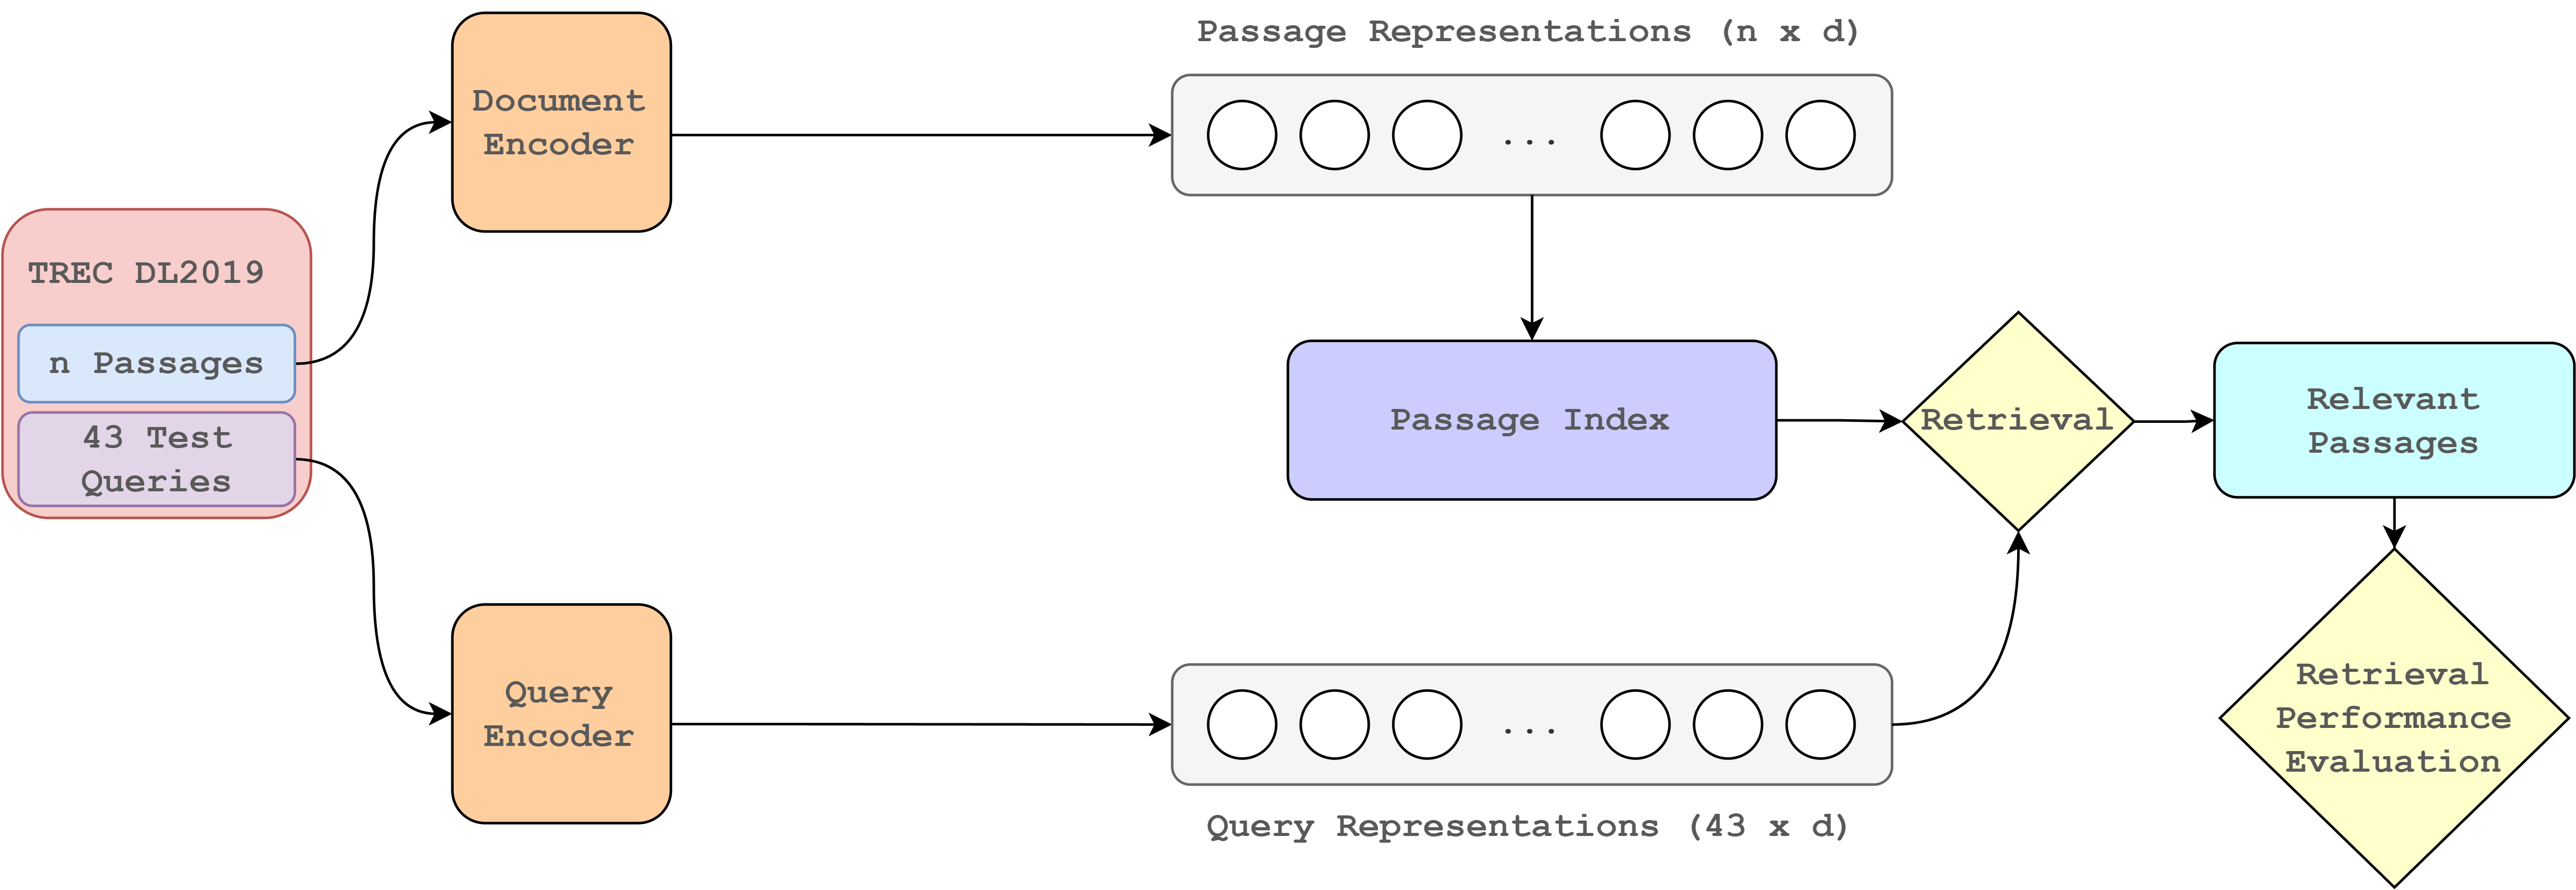
\includegraphics[width=1\textwidth]{figures/IR_Bi_Encoder.png}}
    \end{figure}
    \cite{TREC2019}
\end{frame}

\begin{frame}{Approach -- Causal Probing: Procedure}
    \begin{figure}[!ht]
        \centering
        \makebox[\textwidth][c]{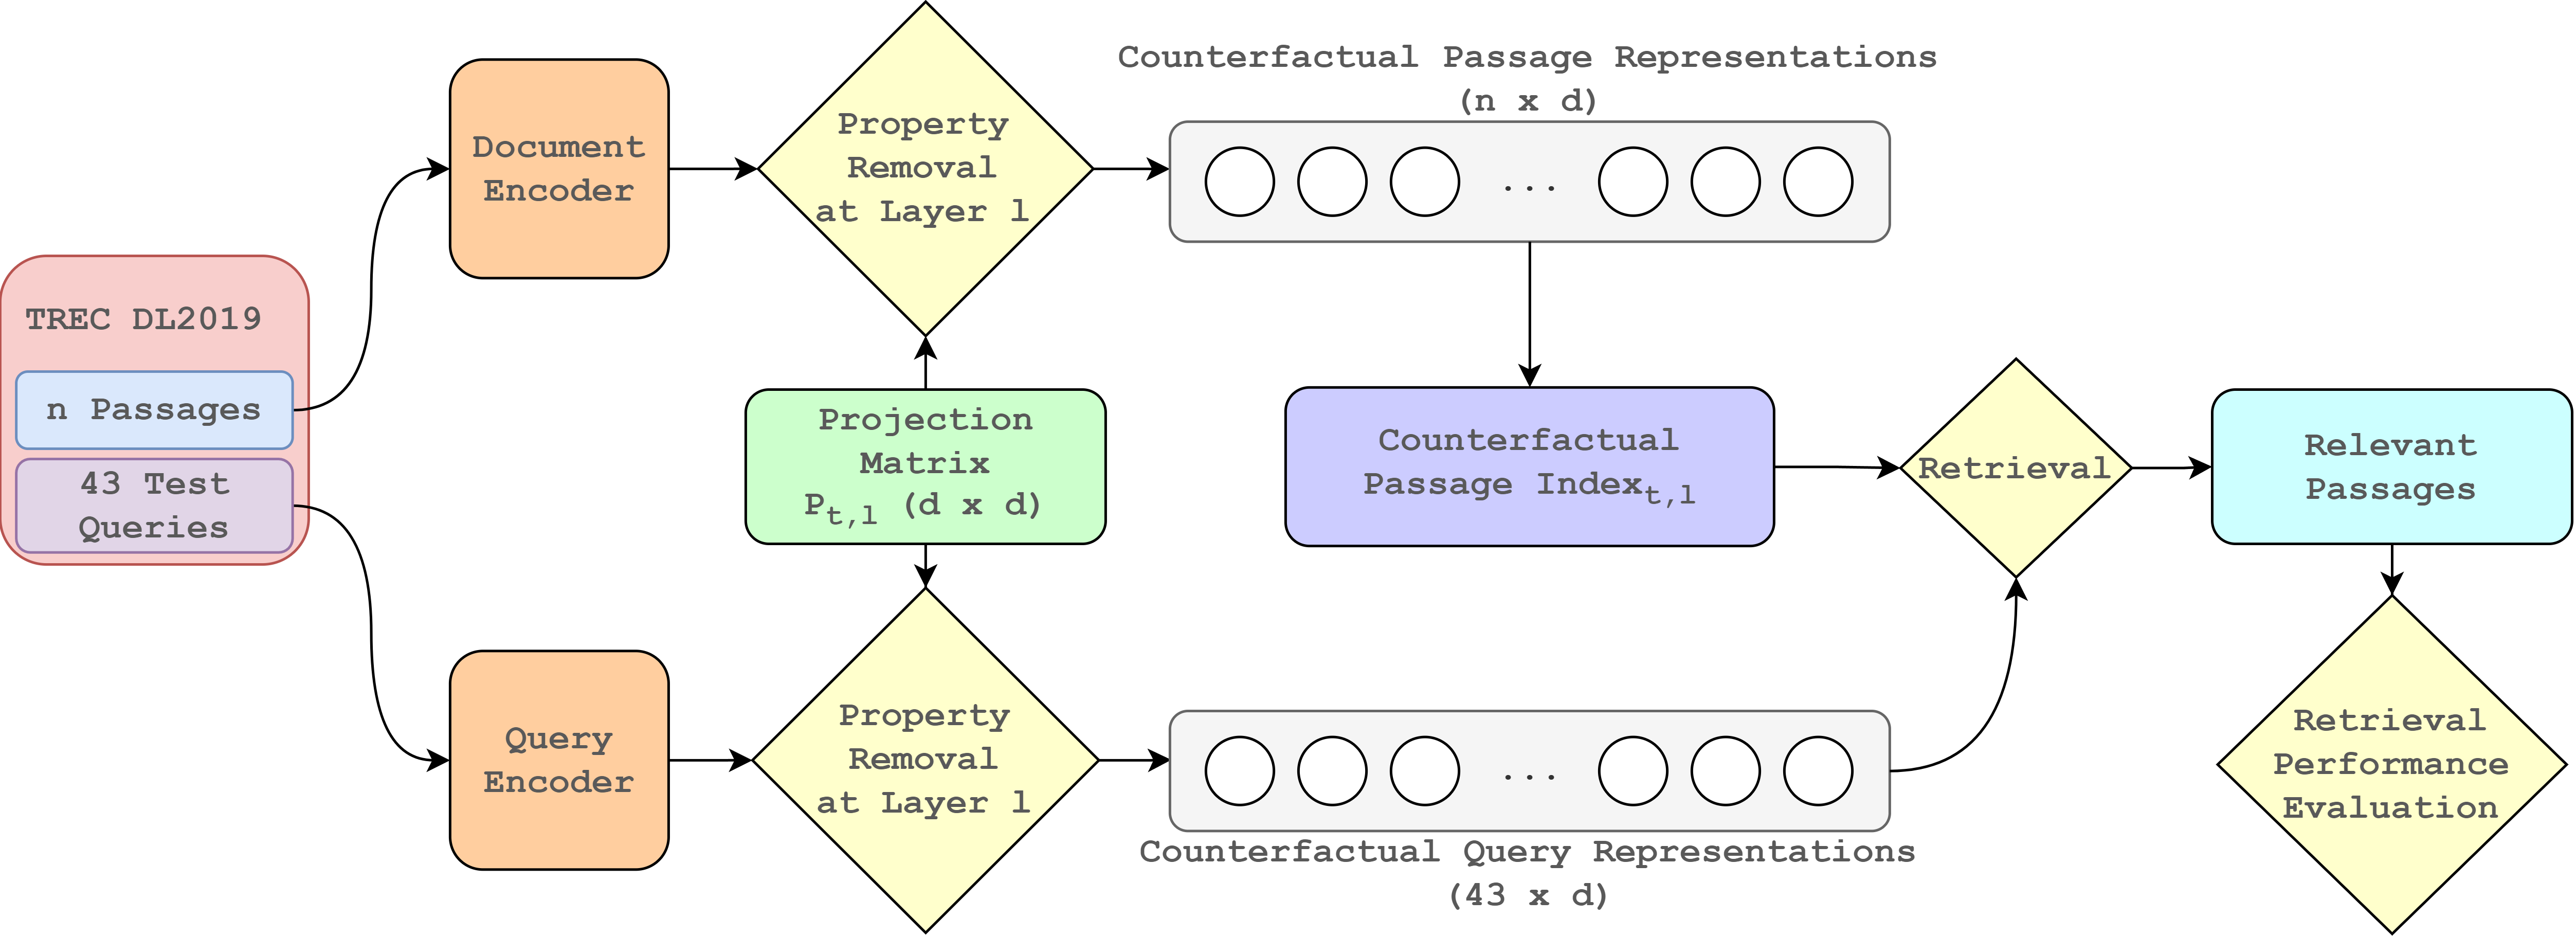
\includegraphics[width=1\textwidth]{figures/Probing_Procedure (2).png}}
    \end{figure}
\end{frame}
% Link: Now that we know the key idea of causal probing and how the counterfactual intervention is done we can define the whole procedure of our approach
% Dataset: TREC 2019 DL Track, 43 Test Queries
% Separate encoding of 8.8M passages and 43 Queries
% Counterfactual Intervention (Property Removal at each layer)
% Passsages are indexed
% Retrieval performed for Test queries to measure performance
% Prodecure differs for QC: Intervention only on queries

\begin{frame}{Approach -- Investigated IR Properties}
    \begin{itemize}
        \item \textbf{BM25}: exact term-matching \cite{bm25} \cite{Robertson1994OkapiAT}
        \item \textbf{SEM}: Semantic similarity of query and document (cosine similarity between averaged GloVe-embeddings \cite{GloVe})
        \item \textbf{TI}: Term importance w.r.t. a query (RSJ weight) \cite{Robertson-Relevance-1976,Formal__match_your_words}
              % \begin{equation}
              %     RSJ(t,q, \mathcal{C}) = \log \frac{p(t|\mathcal{R})p( \neg t | \neg \mathcal{R})}{p(\neg t|\mathcal{R})p( t | \neg \mathcal{R})}
              % \end{equation}
        \item \textbf{NER}: Named-entity recognition
        \item \textbf{COREF}: Coreference resolution
        \item \textbf{QC}: Question classification
    \end{itemize}
\end{frame}
% Token and Sequnce level tasks
% BM25: traditional IR model exact term matching and corpus statistics
% SEM: sort of soft term matching
% TI: Term importance of individual terms considering a query
%   calculated by the Robertson Spärck Jones weight
% NER: 18 classes of entities
% COREF: Coreference of a term within a document
% QC: ABBREVIATION, ENTITY, DESCRIPTION, HUMAN, LOCATION, and NUMERIC VALUE.

\begin{frame}{Approach -- Feasibility Studies}
    \begin{enumerate}
        \item Eliminating Subspaces of Increasing Ranks
              \begin{itemize}
                  \item Goals: Investigate influence of $k$; find the best $k$ for each property
              \end{itemize}
        \item Probing as a Sanity Check
              \begin{itemize}
                  \item Goals: Confirm that properties are linearly encoded in the subject model's representations and R-LACE succesfully removes them
              \end{itemize}
    \end{enumerate}
\end{frame}


\begin{frame}{Results -- Feasibility Study: Eliminating Subspaces of Increasing Ranks}
    Depicted property: Question classification
    \begin{figure}[!ht]
        \centering
        \makebox[\textwidth][c]{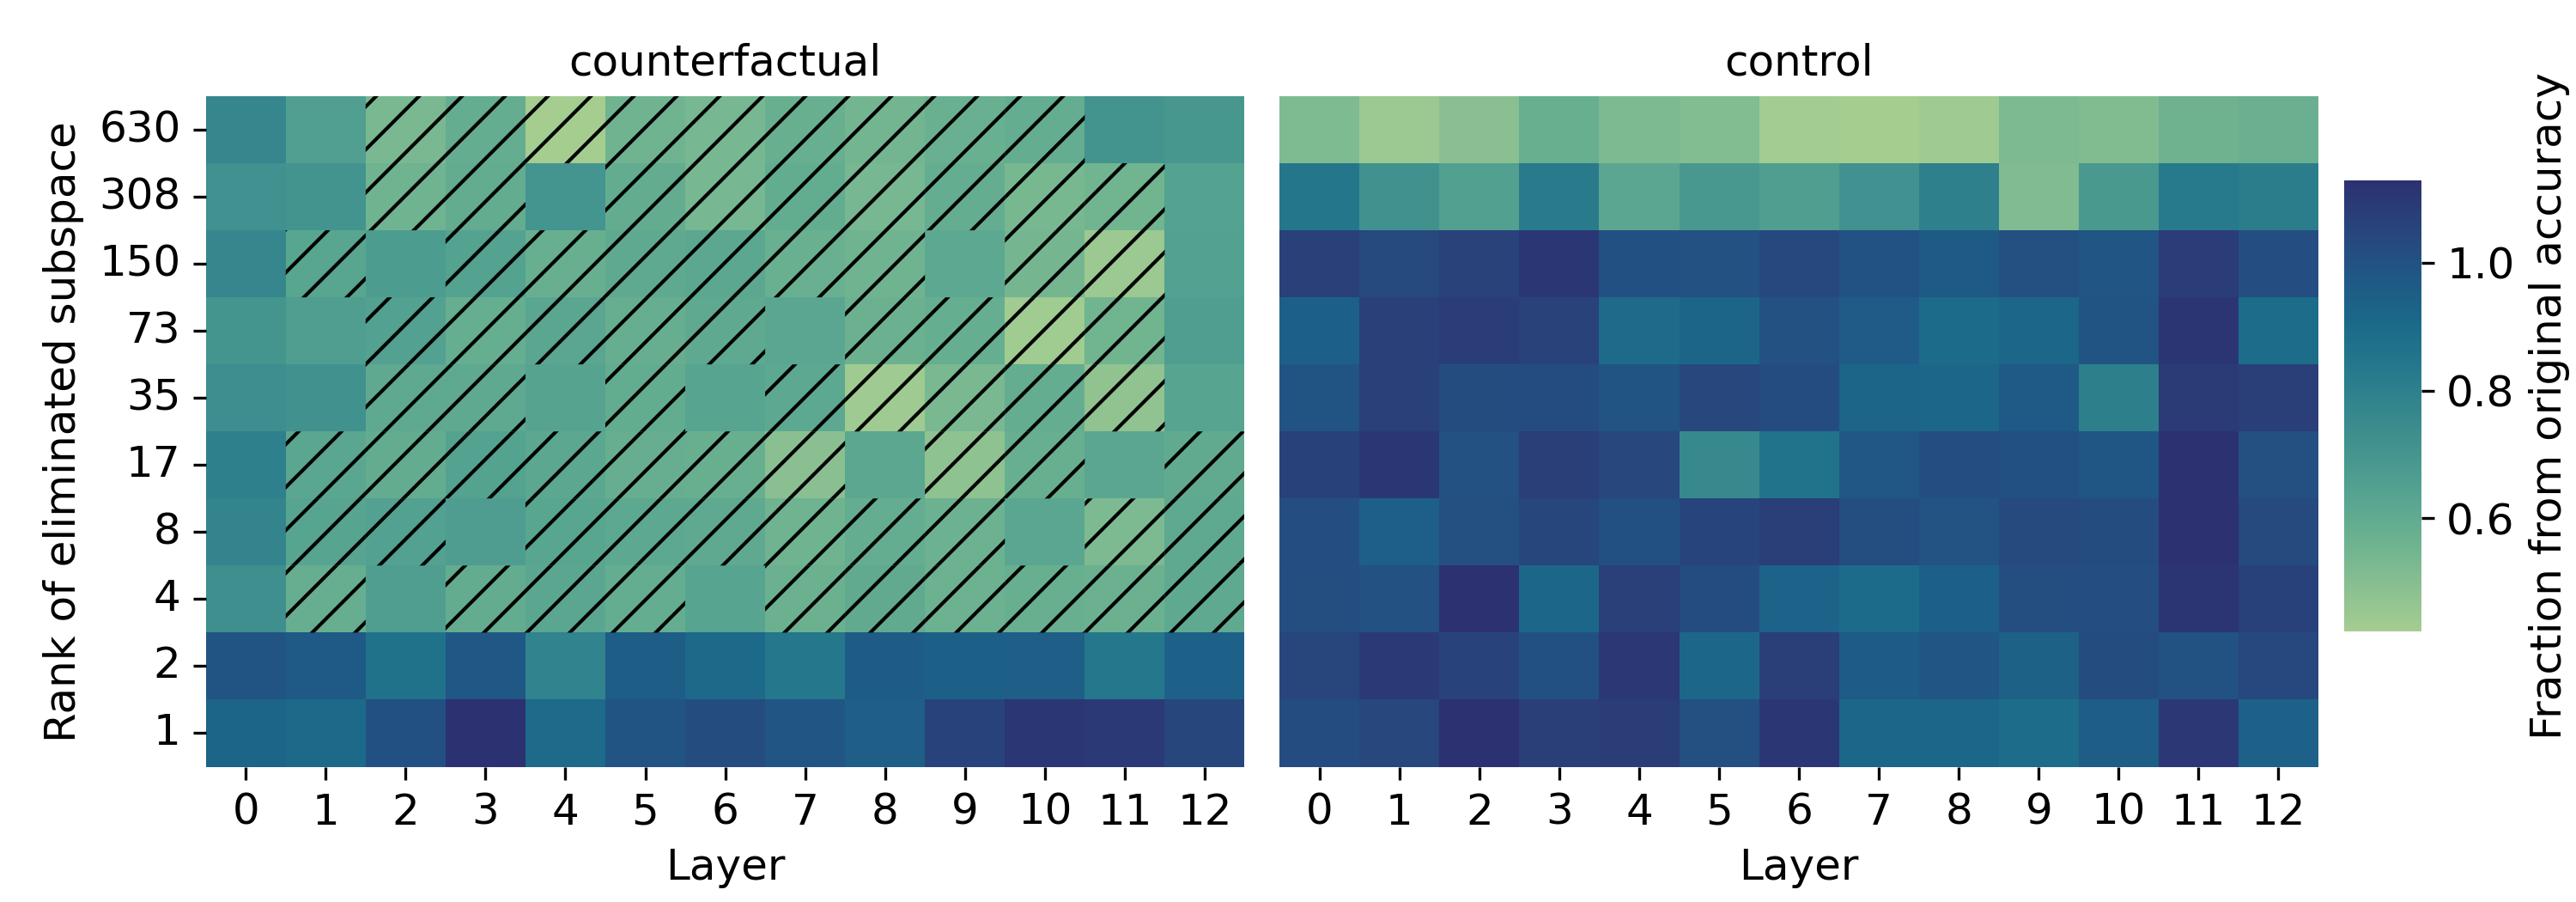
\includegraphics[width=1\textwidth]{figures/qc_coarse_subspace_heatmap.png}}
    \end{figure}
\end{frame}
% Link: 
% For some properties the intervention did not seem to erase the concept (with k=1), which is why we designed this experiment.
% What you see: Fraction of probes accuracy on the task before and after the intervention at every layer with increasing k.
% Darker colors (value of 1) depict no accuracy change through the intervention.
% Stripes indicate where the accuracy is equal or below the majority accuracy.
% Top row: NER, Bottom row: QC
% 

\begin{frame}{Feasibility Study: Probing as a Sanity Check}
    \begin{itemize}
        \item Conventionally probe 3 kinds of representations for each property: original (fixed), counterfactual and control
        \item Sanity check considered passed when accuracies meet the following:
              \begin{enumerate}
                  \item original $>$ majority
                  \item counterfactual $<$ original (preferably counterfactual $\le$ majority)
                  \item counterfactual $<$ control
              \end{enumerate}
    \end{itemize}
\end{frame}

\begin{frame}{Results -- Feasibility Study: Probing as a Sanity Check (1/3)}
    \begin{figure}[!ht]
        \centering
        \makebox[\textwidth][c]{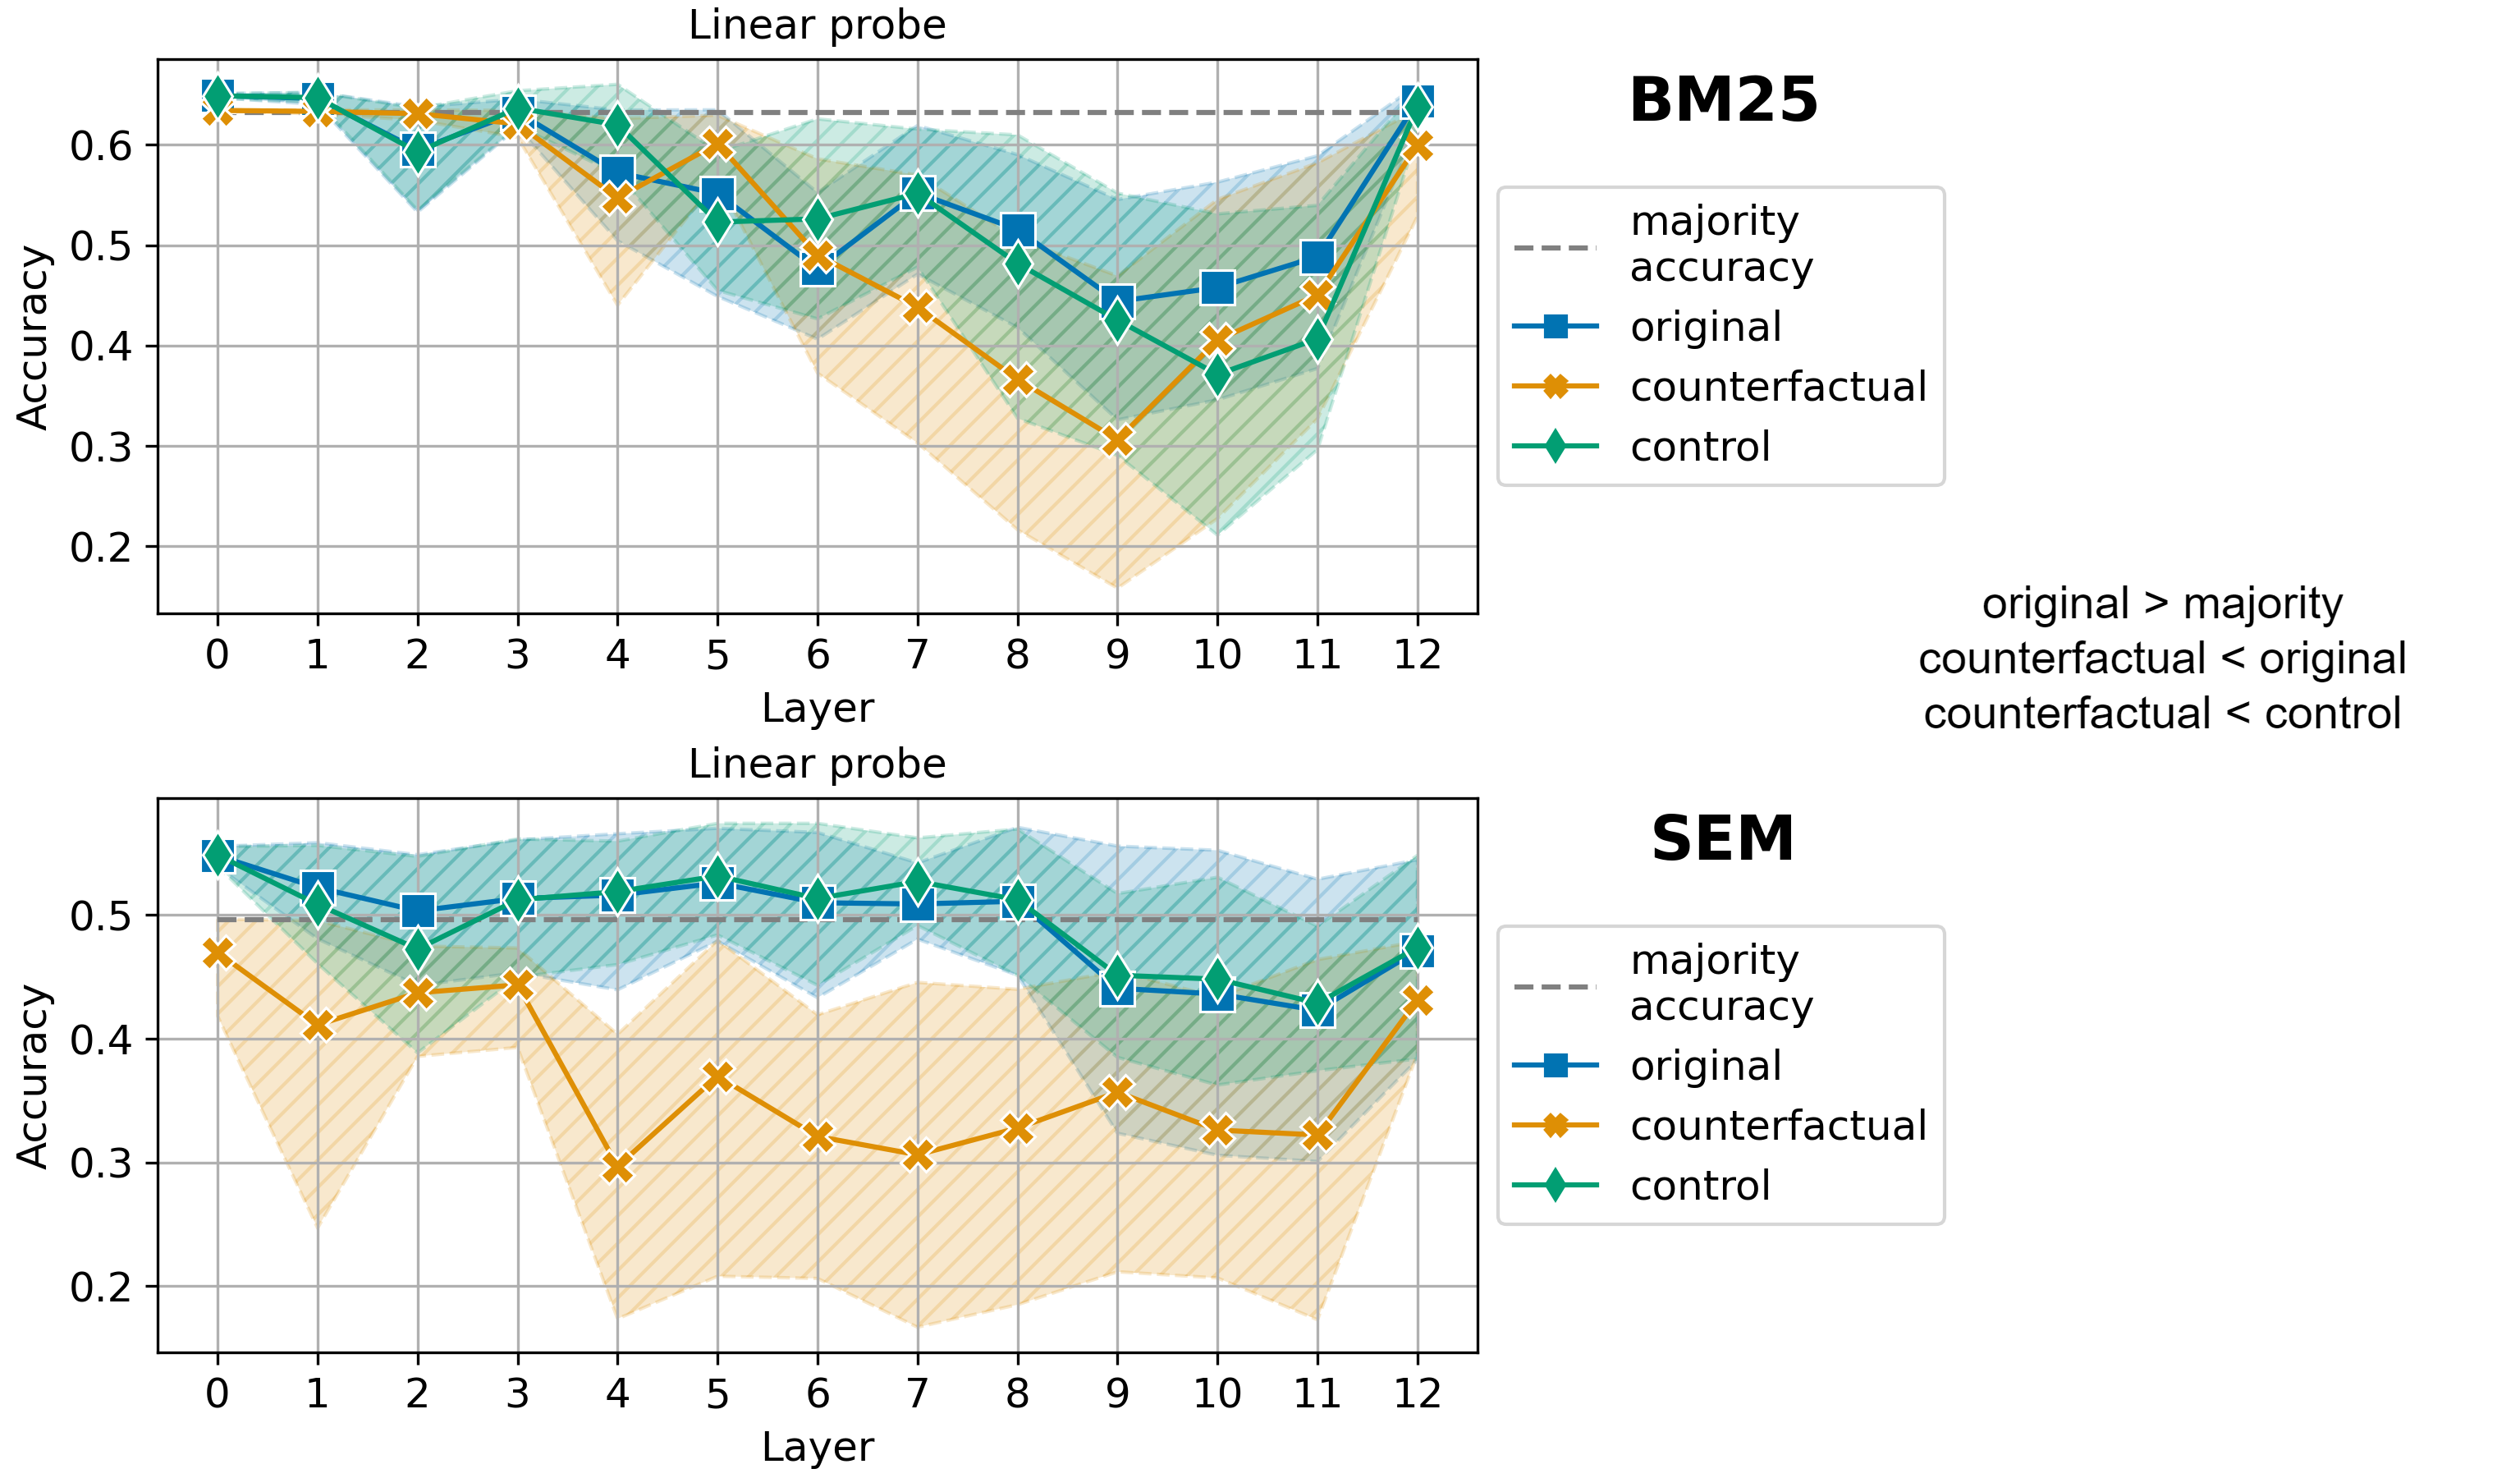
\includegraphics[width=0.9\textwidth]{figures/sanity_check/bm25_sem (1).png}}
    \end{figure}
\end{frame}

\begin{frame}{Results -- Feasibility Study: Probing as a Sanity Check (2/3)}
    \begin{figure}[!ht]
        \centering
        \makebox[\textwidth][c]{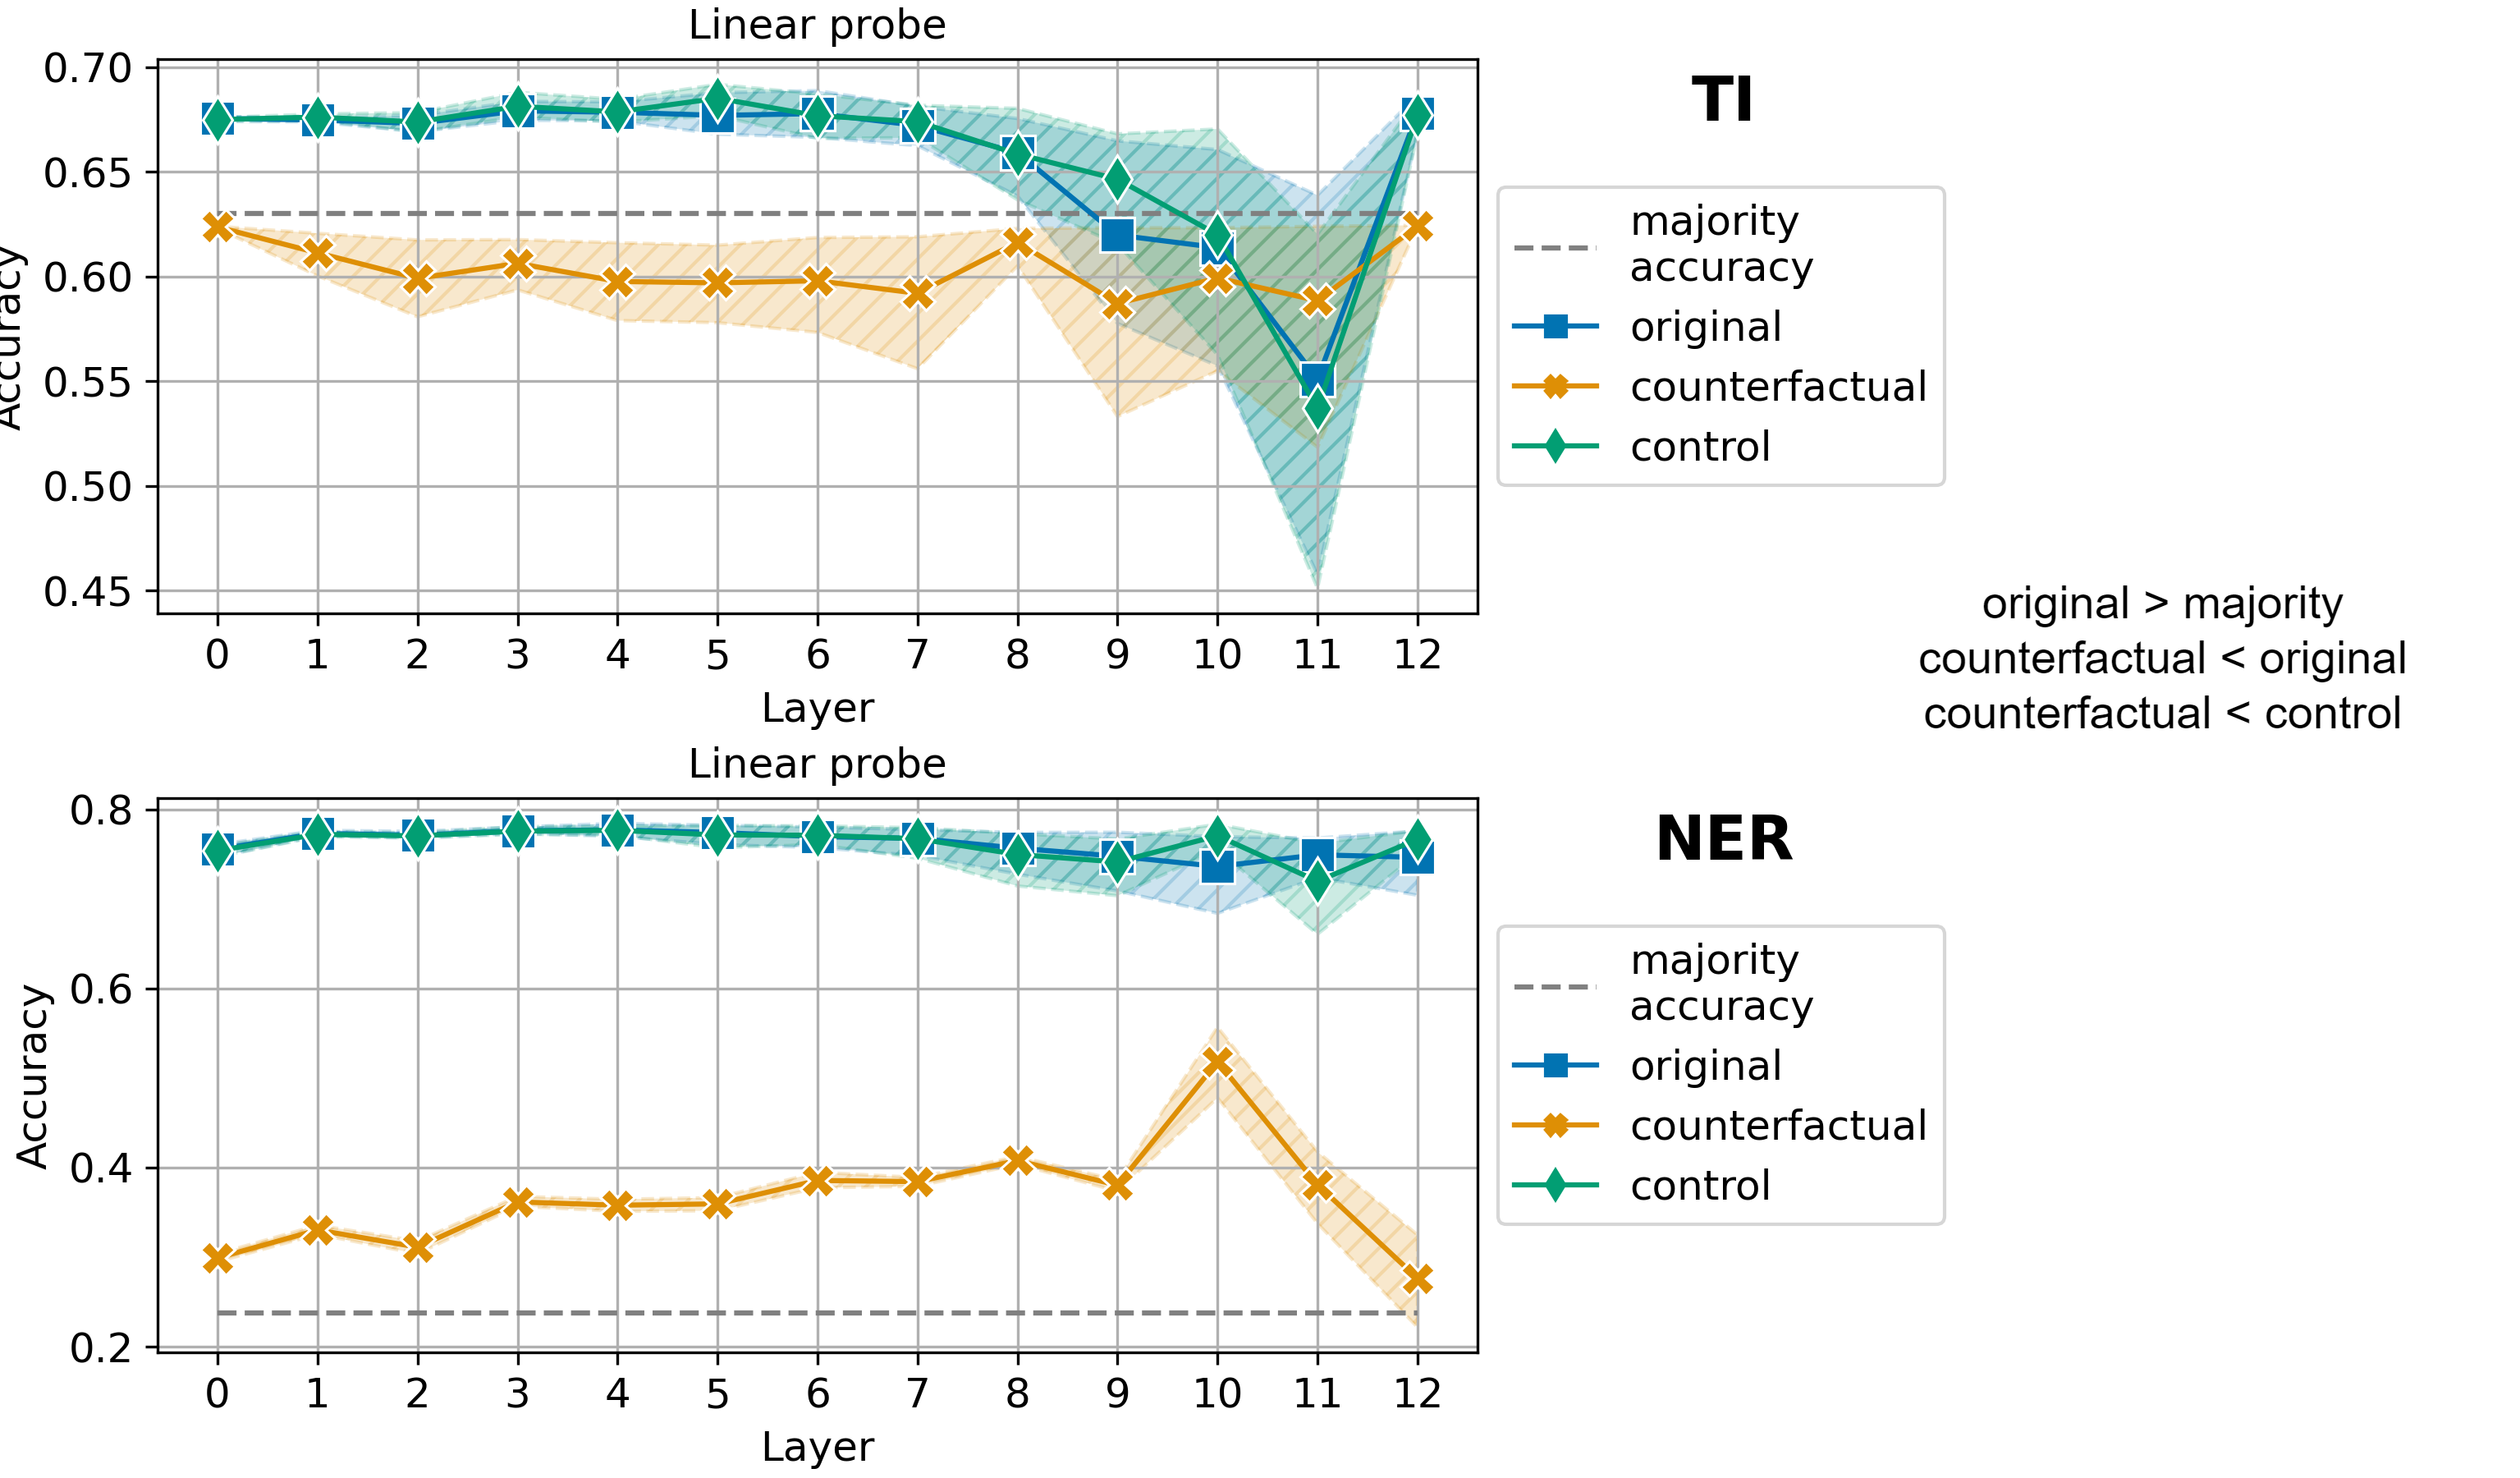
\includegraphics[width=0.9\textwidth]{figures/sanity_check/ti_ner (1).png}}
    \end{figure}
\end{frame}

\begin{frame}{Results -- Feasibility Study: Probing as a Sanity Check (3/3)}
    \begin{figure}[!ht]
        \centering
        \makebox[\textwidth][c]{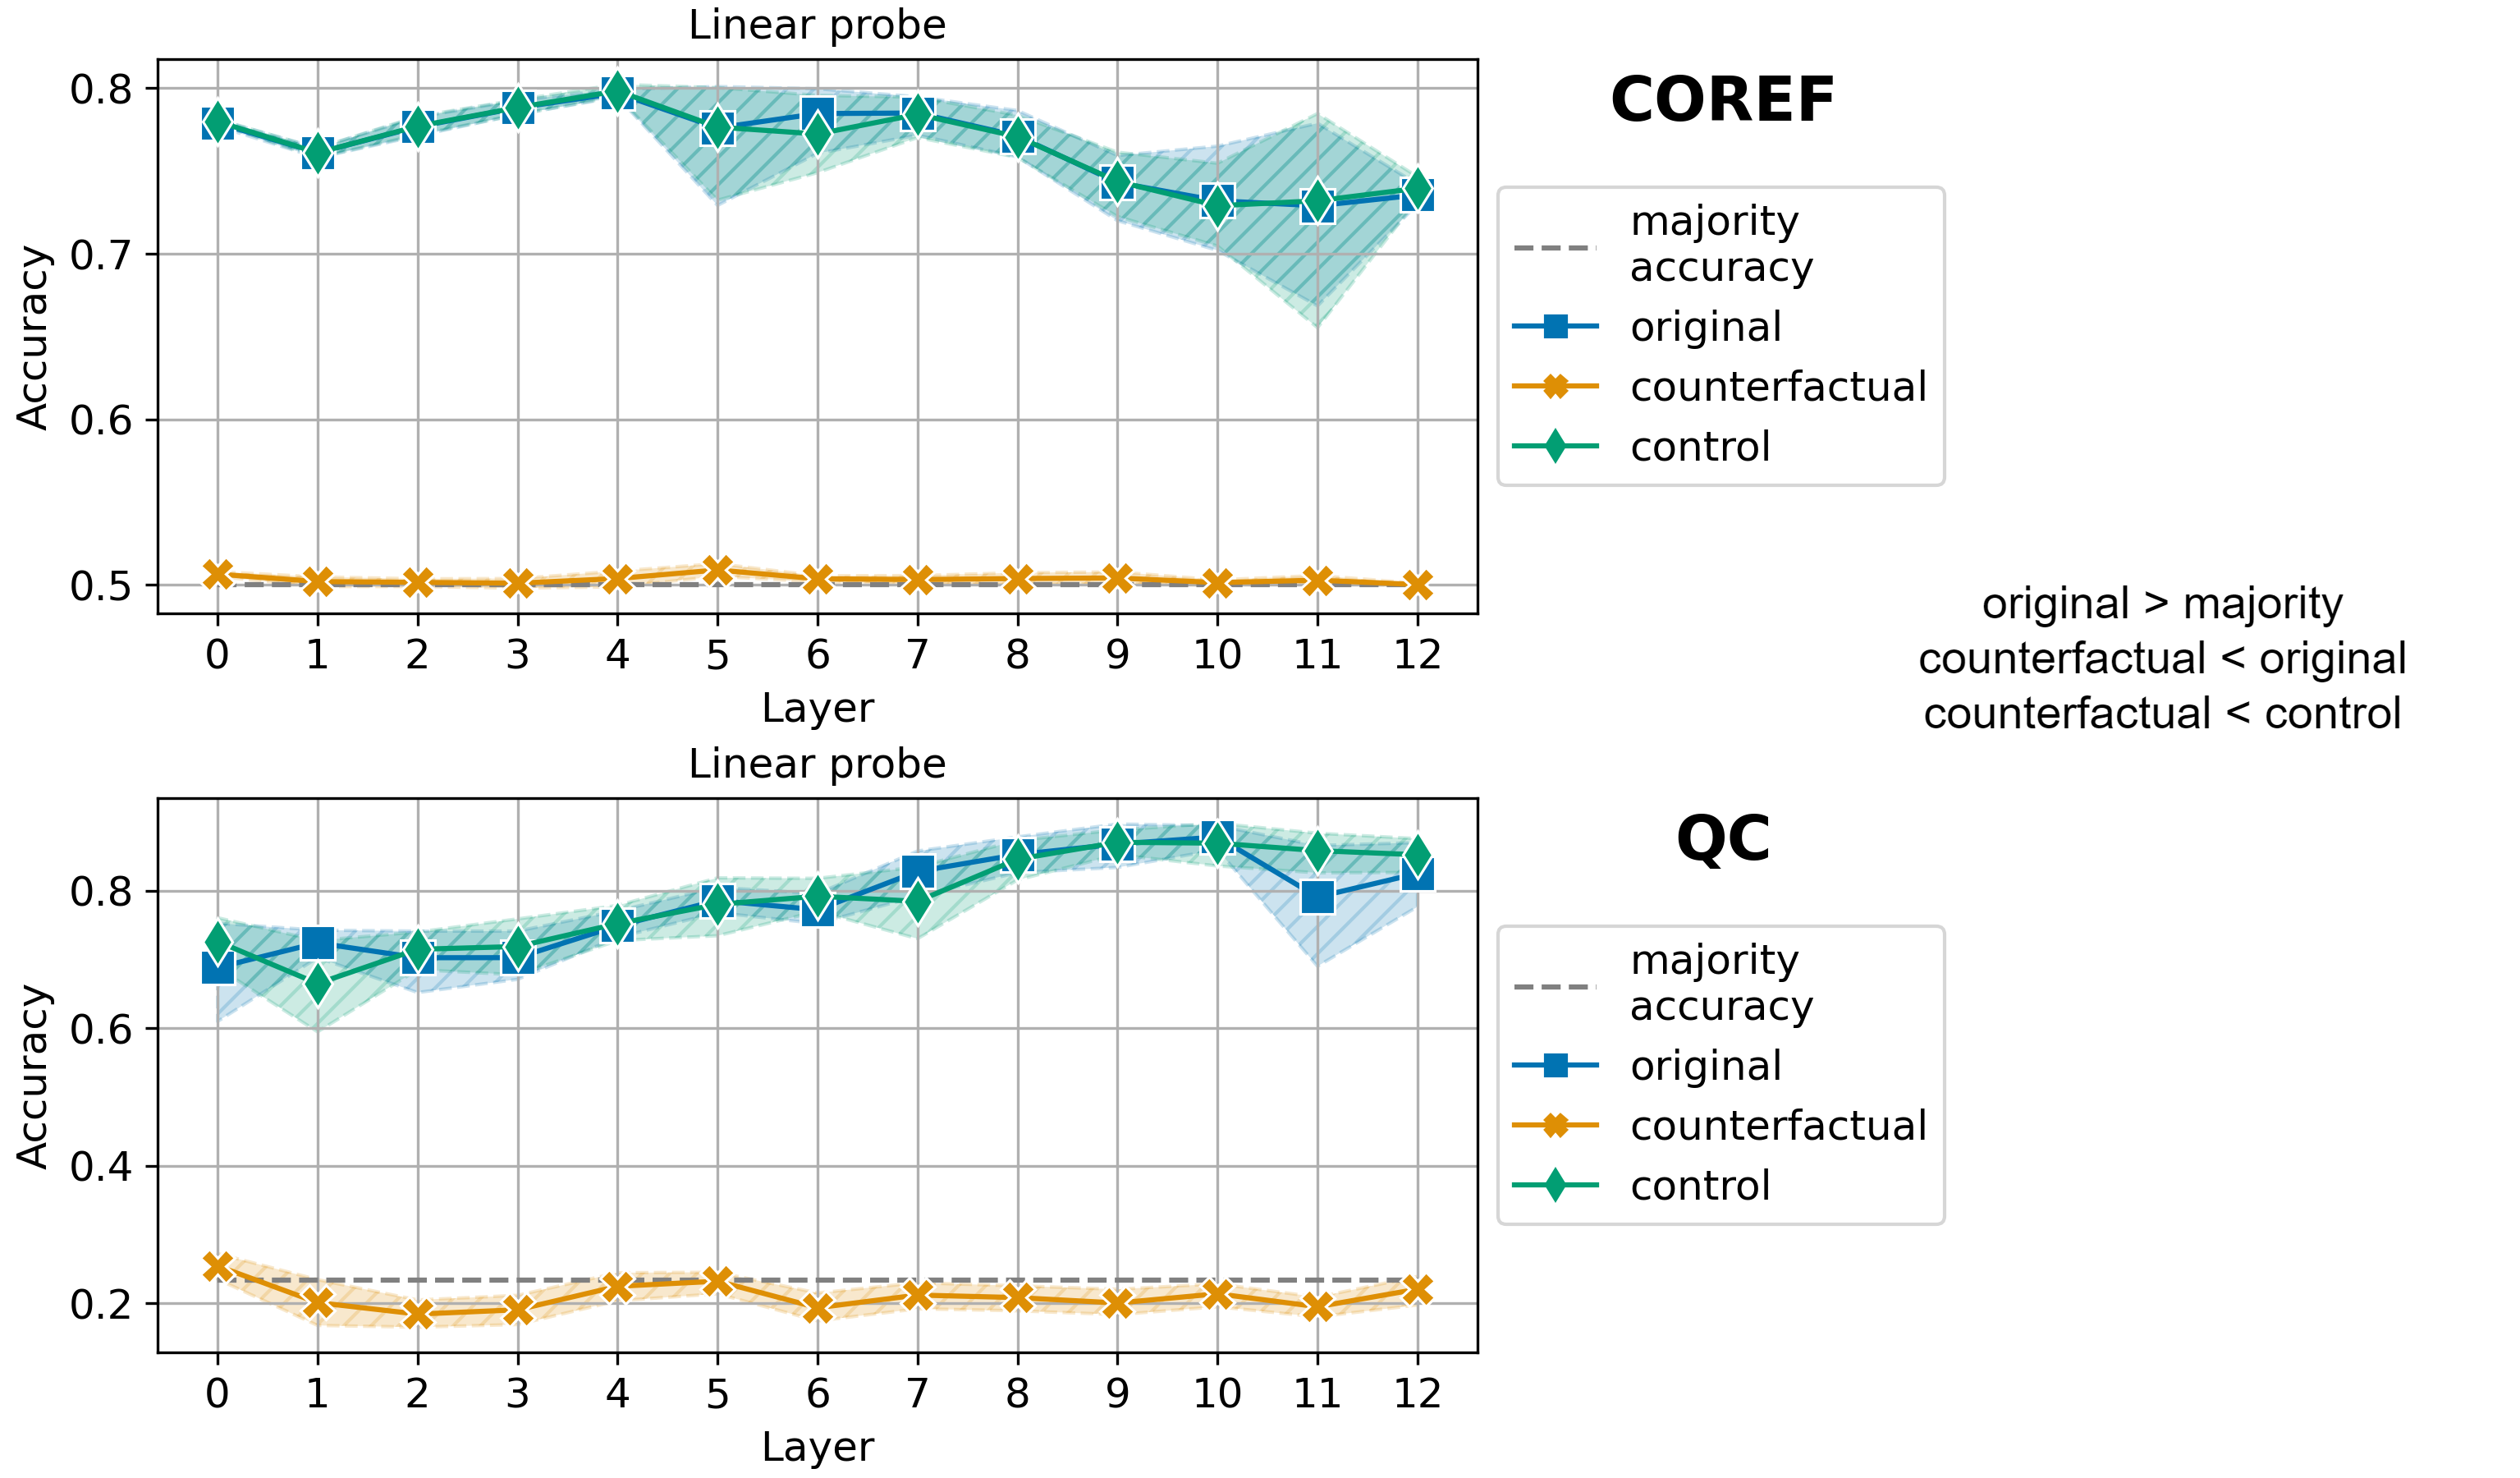
\includegraphics[width=0.9\textwidth]{figures/sanity_check/core_qc.png}}
    \end{figure}
\end{frame}

\begin{frame}{Results -- Causal Probing}
    \begin{figure}[!ht]
        \centering
        \makebox[\textwidth][c]{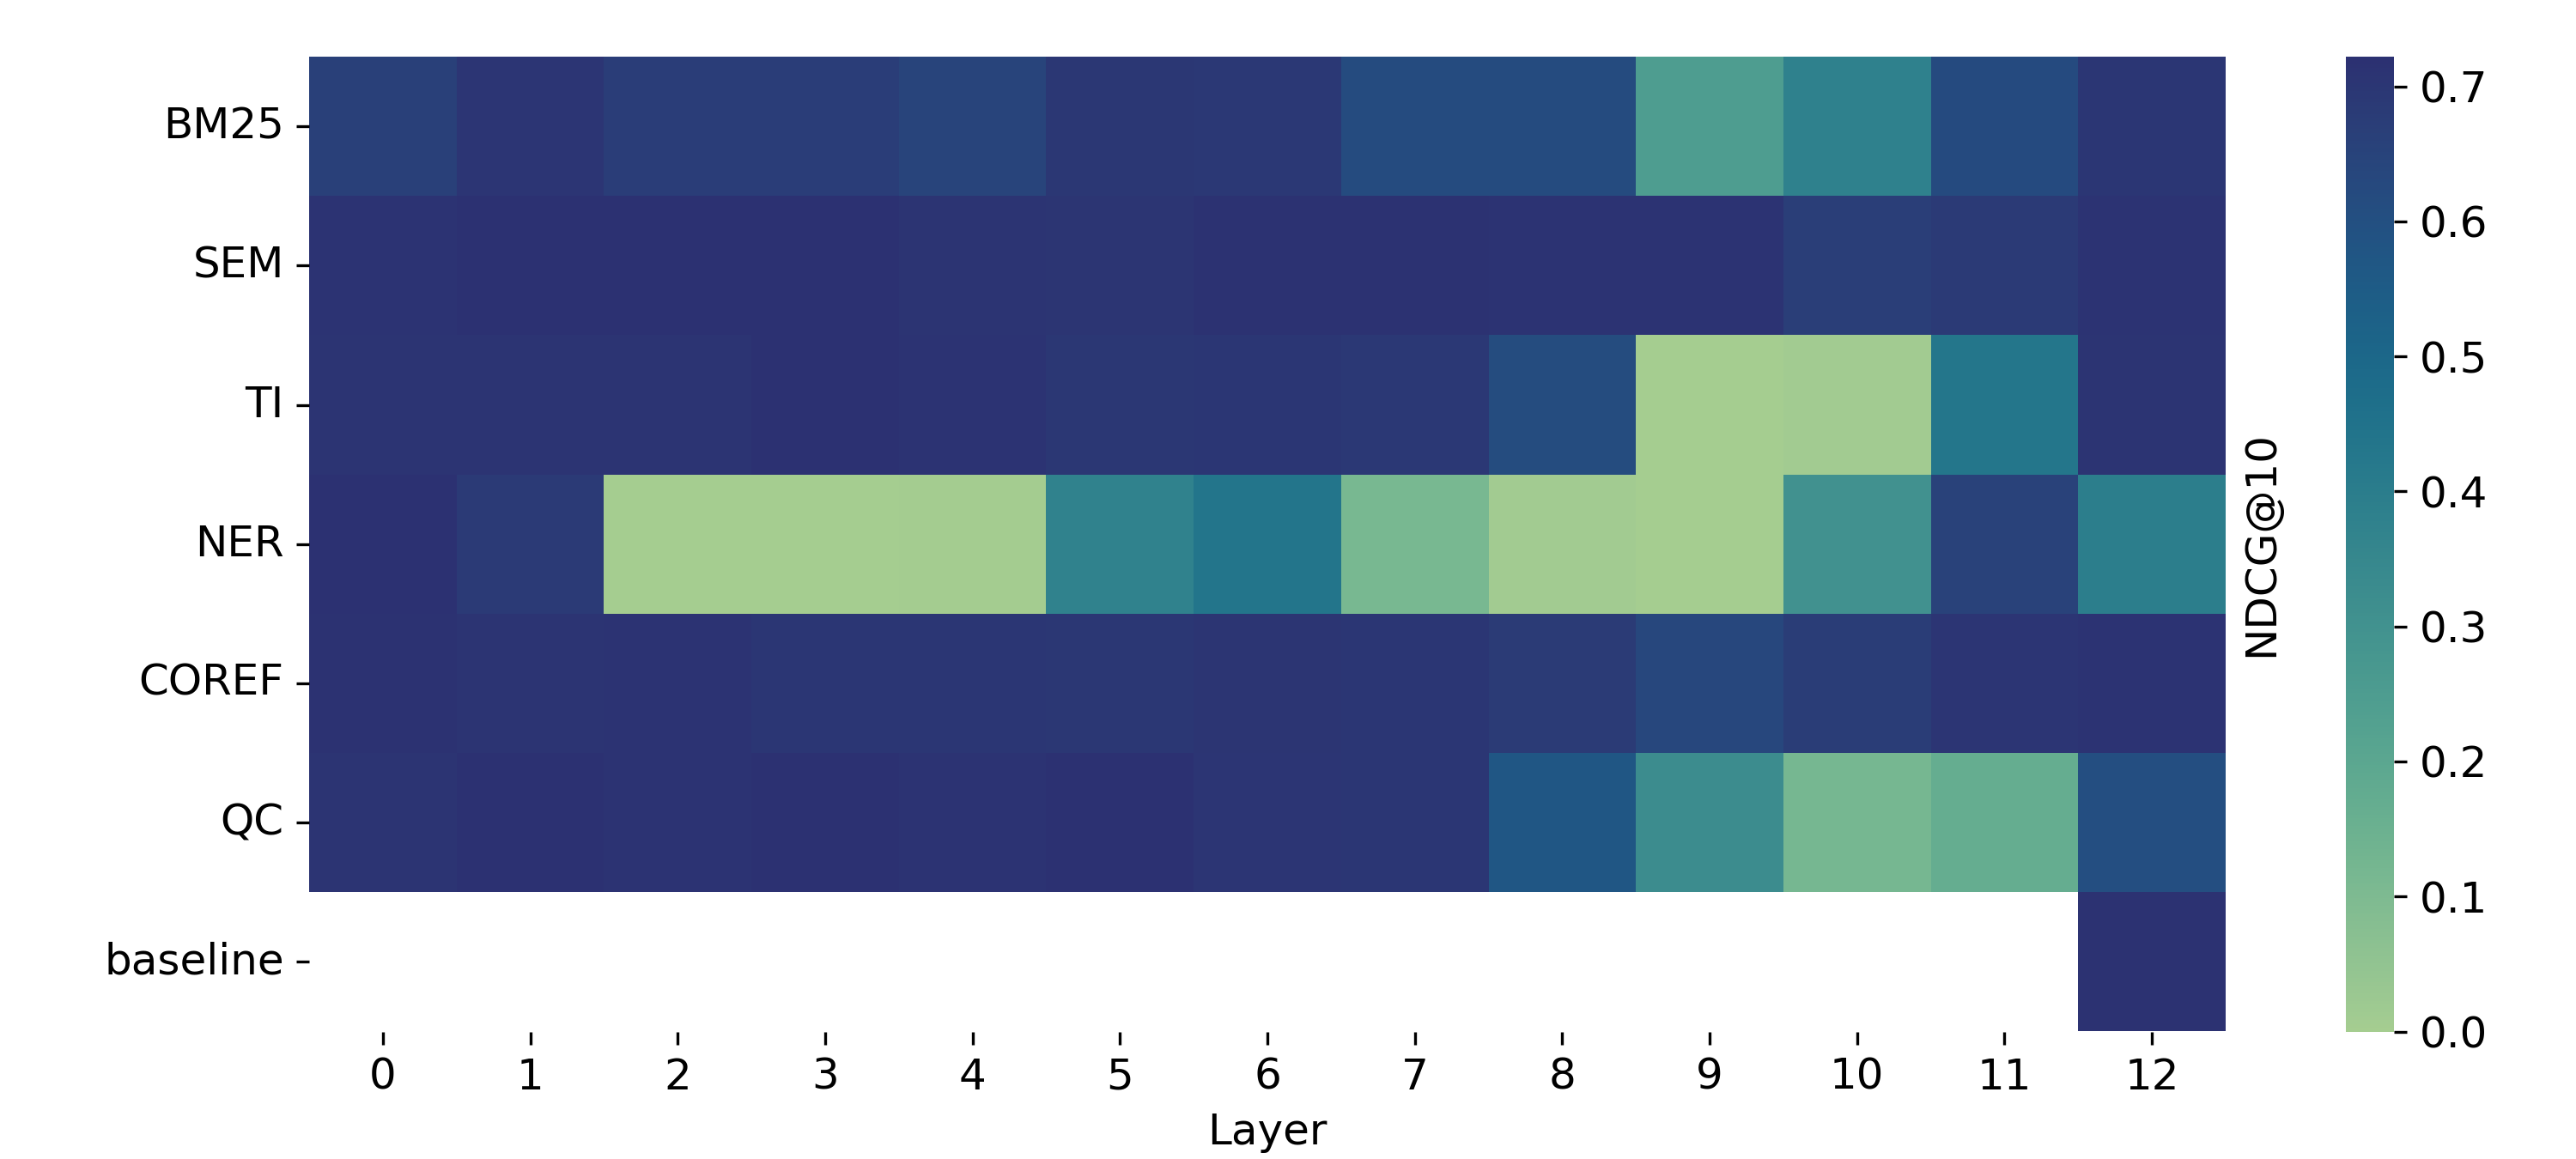
\includegraphics[width=1\textwidth]{figures/all_behaviour_heatmap_ndcg_10_shortened.png}}
    \end{figure}
\end{frame}


\begin{frame}{Conclusion (1/2)}
    \begin{itemize}
        \item \scriptsize{\textbf{RQ1} Can we confirm the feasibility of \textit{causally probing} our bi-encoder subject model in the context of retrieval?}
              \begin{itemize}
                  \item Yes, for most of the properties. Limitations for BM25 and SEM.
              \end{itemize}
        \item \scriptsize{\textbf{RQ2} On which properties does our bi-encoder rely upon to solve the task of text retrieval?}
              \begin{itemize}
                  \item Importance hierarchy: SEM, COREF $<$ BM25, QC $<$ TI, NER
              \end{itemize}
        \item \scriptsize{\textbf{RQ3} At which layers are important properties encoded?}
              \begin{itemize}
                  \item Removal has larger impact at later layers, except for NER.
              \end{itemize}
    \end{itemize}
\end{frame}

\begin{frame}{Conclusion (2/2)}
    \begin{itemize}
        \item \large Limitations:
              \begin{itemize}
                  \item Only approximation of a property gets removed
                  \item Spurious correlations with a property
                  \item Only removal of linear information
              \end{itemize}
        \item \large Future Work:
              \begin{itemize}
                  \item Additional properties
                  \item Investigate other bi-encoder architectures and training regimes
                  \item Use non-linear removal technique \cite{Kernelized_concept_Erasure}
                  \item Use advancement of R-LACE: LEAst-squares Concept Erasure (LEACE) \cite{leace} (closed-form solution for complete linear concept erasure)
              \end{itemize}
    \end{itemize}
\end{frame}

\begin{frame}[allowframebreaks]
    \frametitle{References}
    \bibliographystyle{unsrtnat}
    \bibliography{references.bib}
\end{frame}

\begin{frame}{}
    \textbf{Backup Slides}
\end{frame}

\begin{frame}{ColBERT \cite{colbert}}
    \begin{figure}[!ht]
        \centering
        \makebox[\textwidth][c]{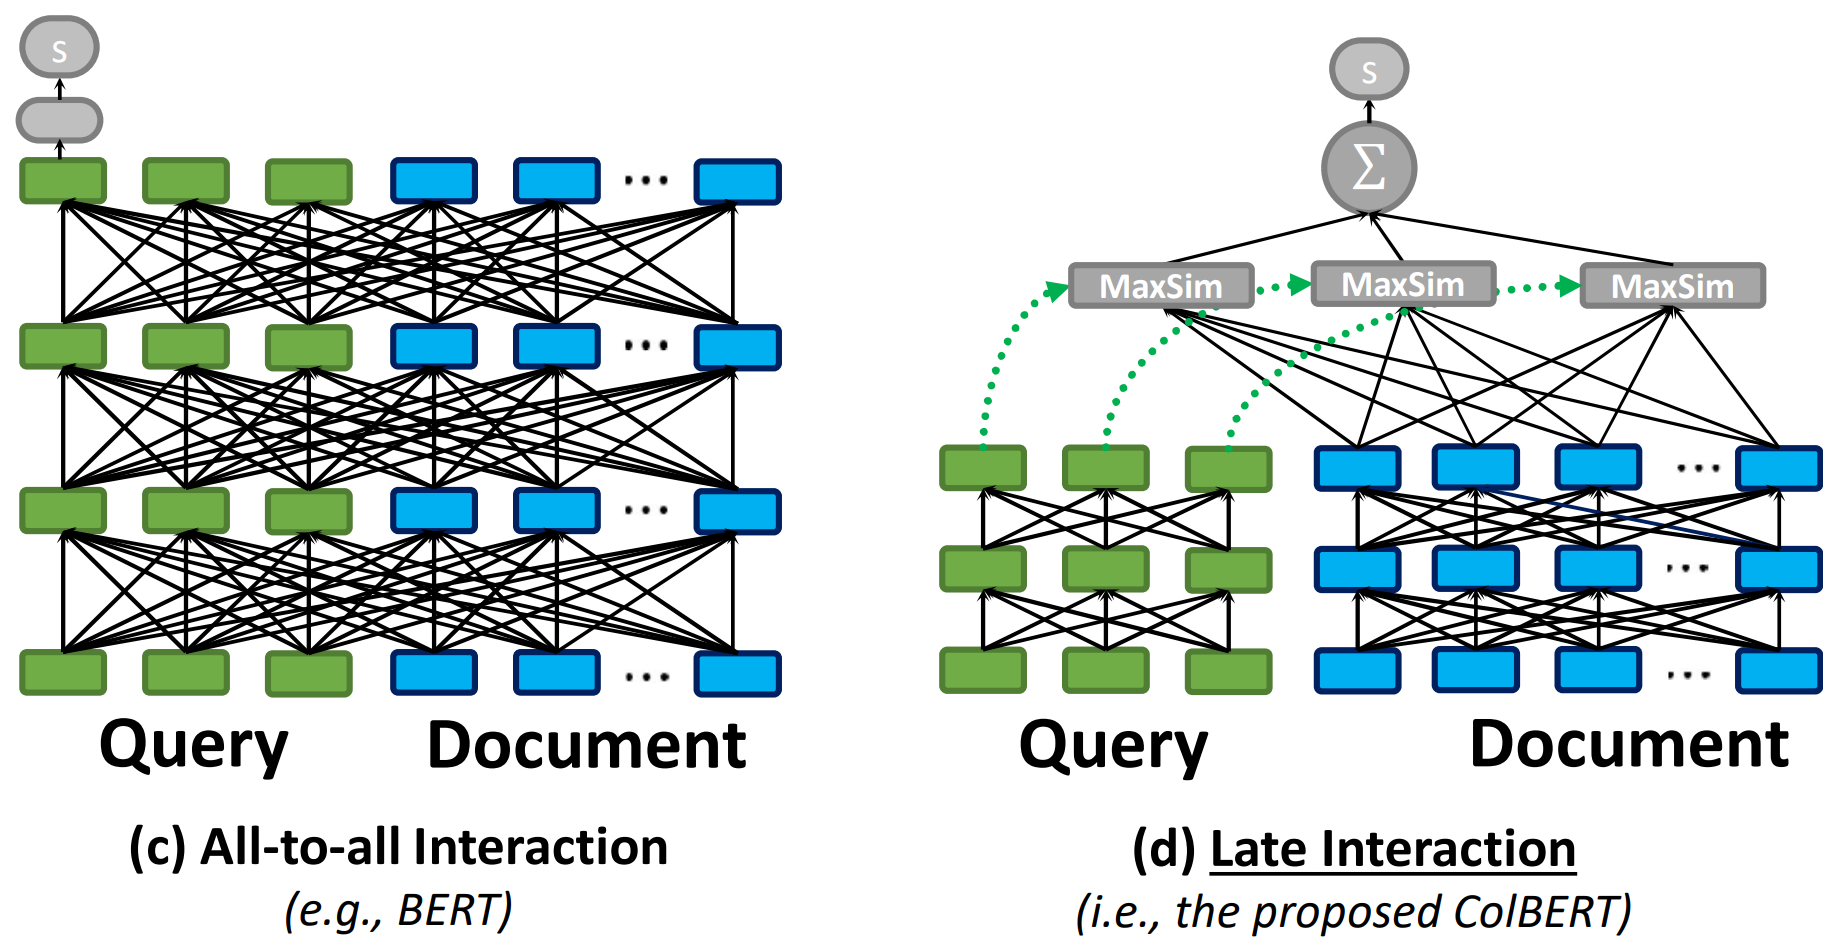
\includegraphics[width=0.9\textwidth]{figures/Colbert.png}}
    \end{figure}
\end{frame}

\begin{frame}{TCT-ColBERT \cite{tct_colbert,tct_colbert2}}
    \begin{figure}[!ht]
        \centering
        \makebox[\textwidth][c]{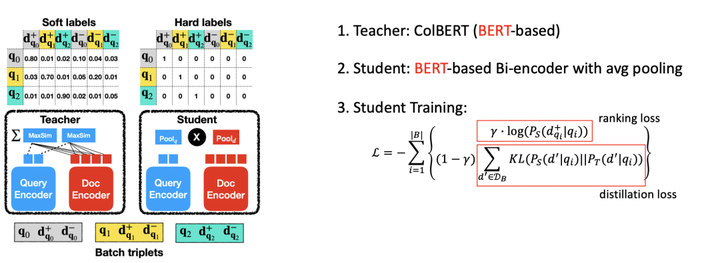
\includegraphics[width=0.9\textwidth]{figures/v2-6be67306ed2b8fa0423ae1db4c3c9d25_720w.png}}
    \end{figure}
    tight coupling: inference with the teacher while distillation, not beforehand
\end{frame}

\begin{frame}{IR Properties -- Examples}
    \begin{figure}[!ht]
        \centering
        \makebox[\textwidth][c]{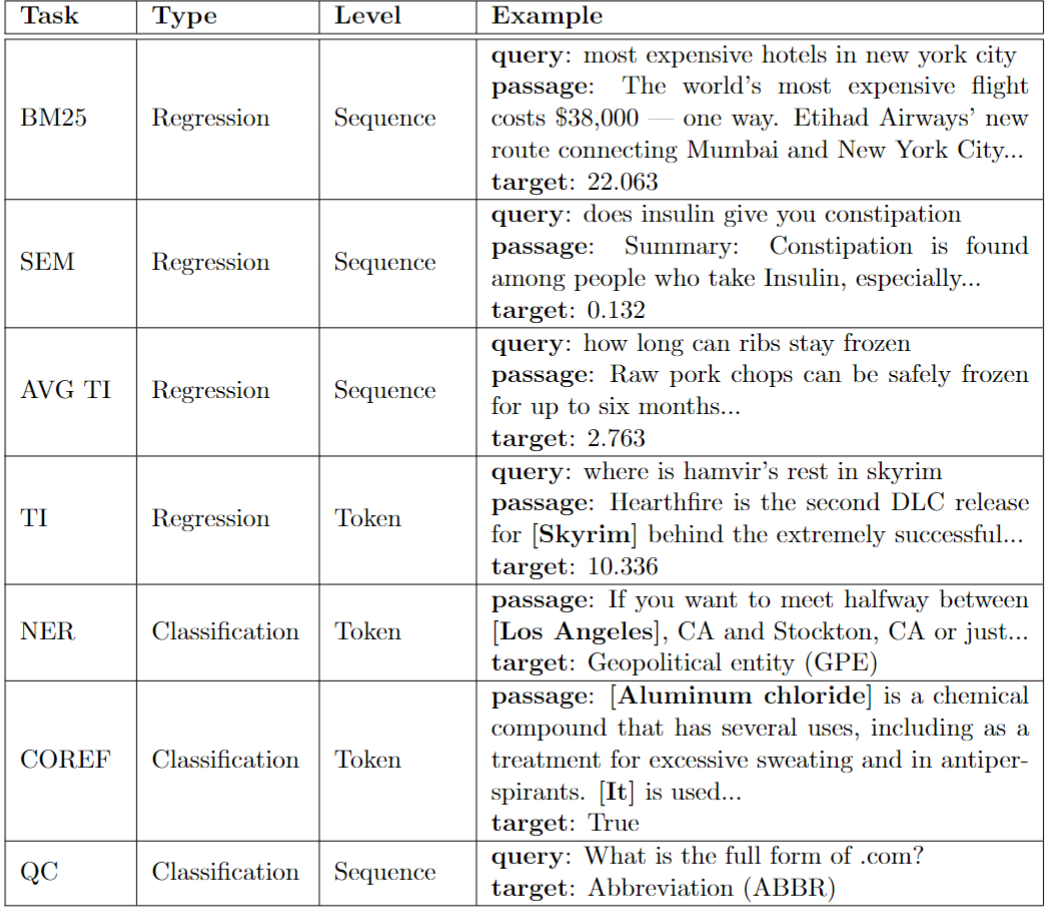
\includegraphics[width=0.65\textwidth]{figures/table_ir_properties.png}}
    \end{figure}
\end{frame}

\begin{frame}{Linear Probe}
    \begin{itemize}
        \item Binary or multinomial logistic regression model, depending on the task
        \item optimization goal (multinomial): \begin{equation}
                  \min_{w, b} - \frac{1}{N} \sum_{i=1}^N\sum_{k=1}^K y_{i,k} \log \frac{\exp(x_iw^{(k)} + b^{(k)})}{\sum_{j=1}^K \exp(x_iw^{(j)} + b^{(j)})}
              \end{equation}
    \end{itemize}
\end{frame}

\begin{frame}{NDCG}
    \begin{itemize}
        \item main metric in TREC DL
        \item \begin{equation}
                  \textrm{NDCG}= \frac{\textrm{DCG}}{\textrm{IDCG}}
              \end{equation}
        \item \begin{equation}
                  \textrm{DCG} = \sum_{i=1}^{|\mathcal{C}|} \frac{y_i}{\log_2(i + 1)}
              \end{equation}
    \end{itemize}
\end{frame}

\begin{frame}{Term Importance -- RSJ formula \cite{Formal__match_your_words}}
    \begin{equation}
        RSJ(t,q, \mathcal{C}) = \log \frac{p(t|\mathcal{R})p( \neg t | \neg \mathcal{R})}{p(\neg t|\mathcal{R})p( t | \neg \mathcal{R})}
    \end{equation}
\end{frame}

\begin{frame}{Causal Probing Results -- Recall@1000}
    \begin{figure}[!ht]
        \centering
        \makebox[\textwidth][c]{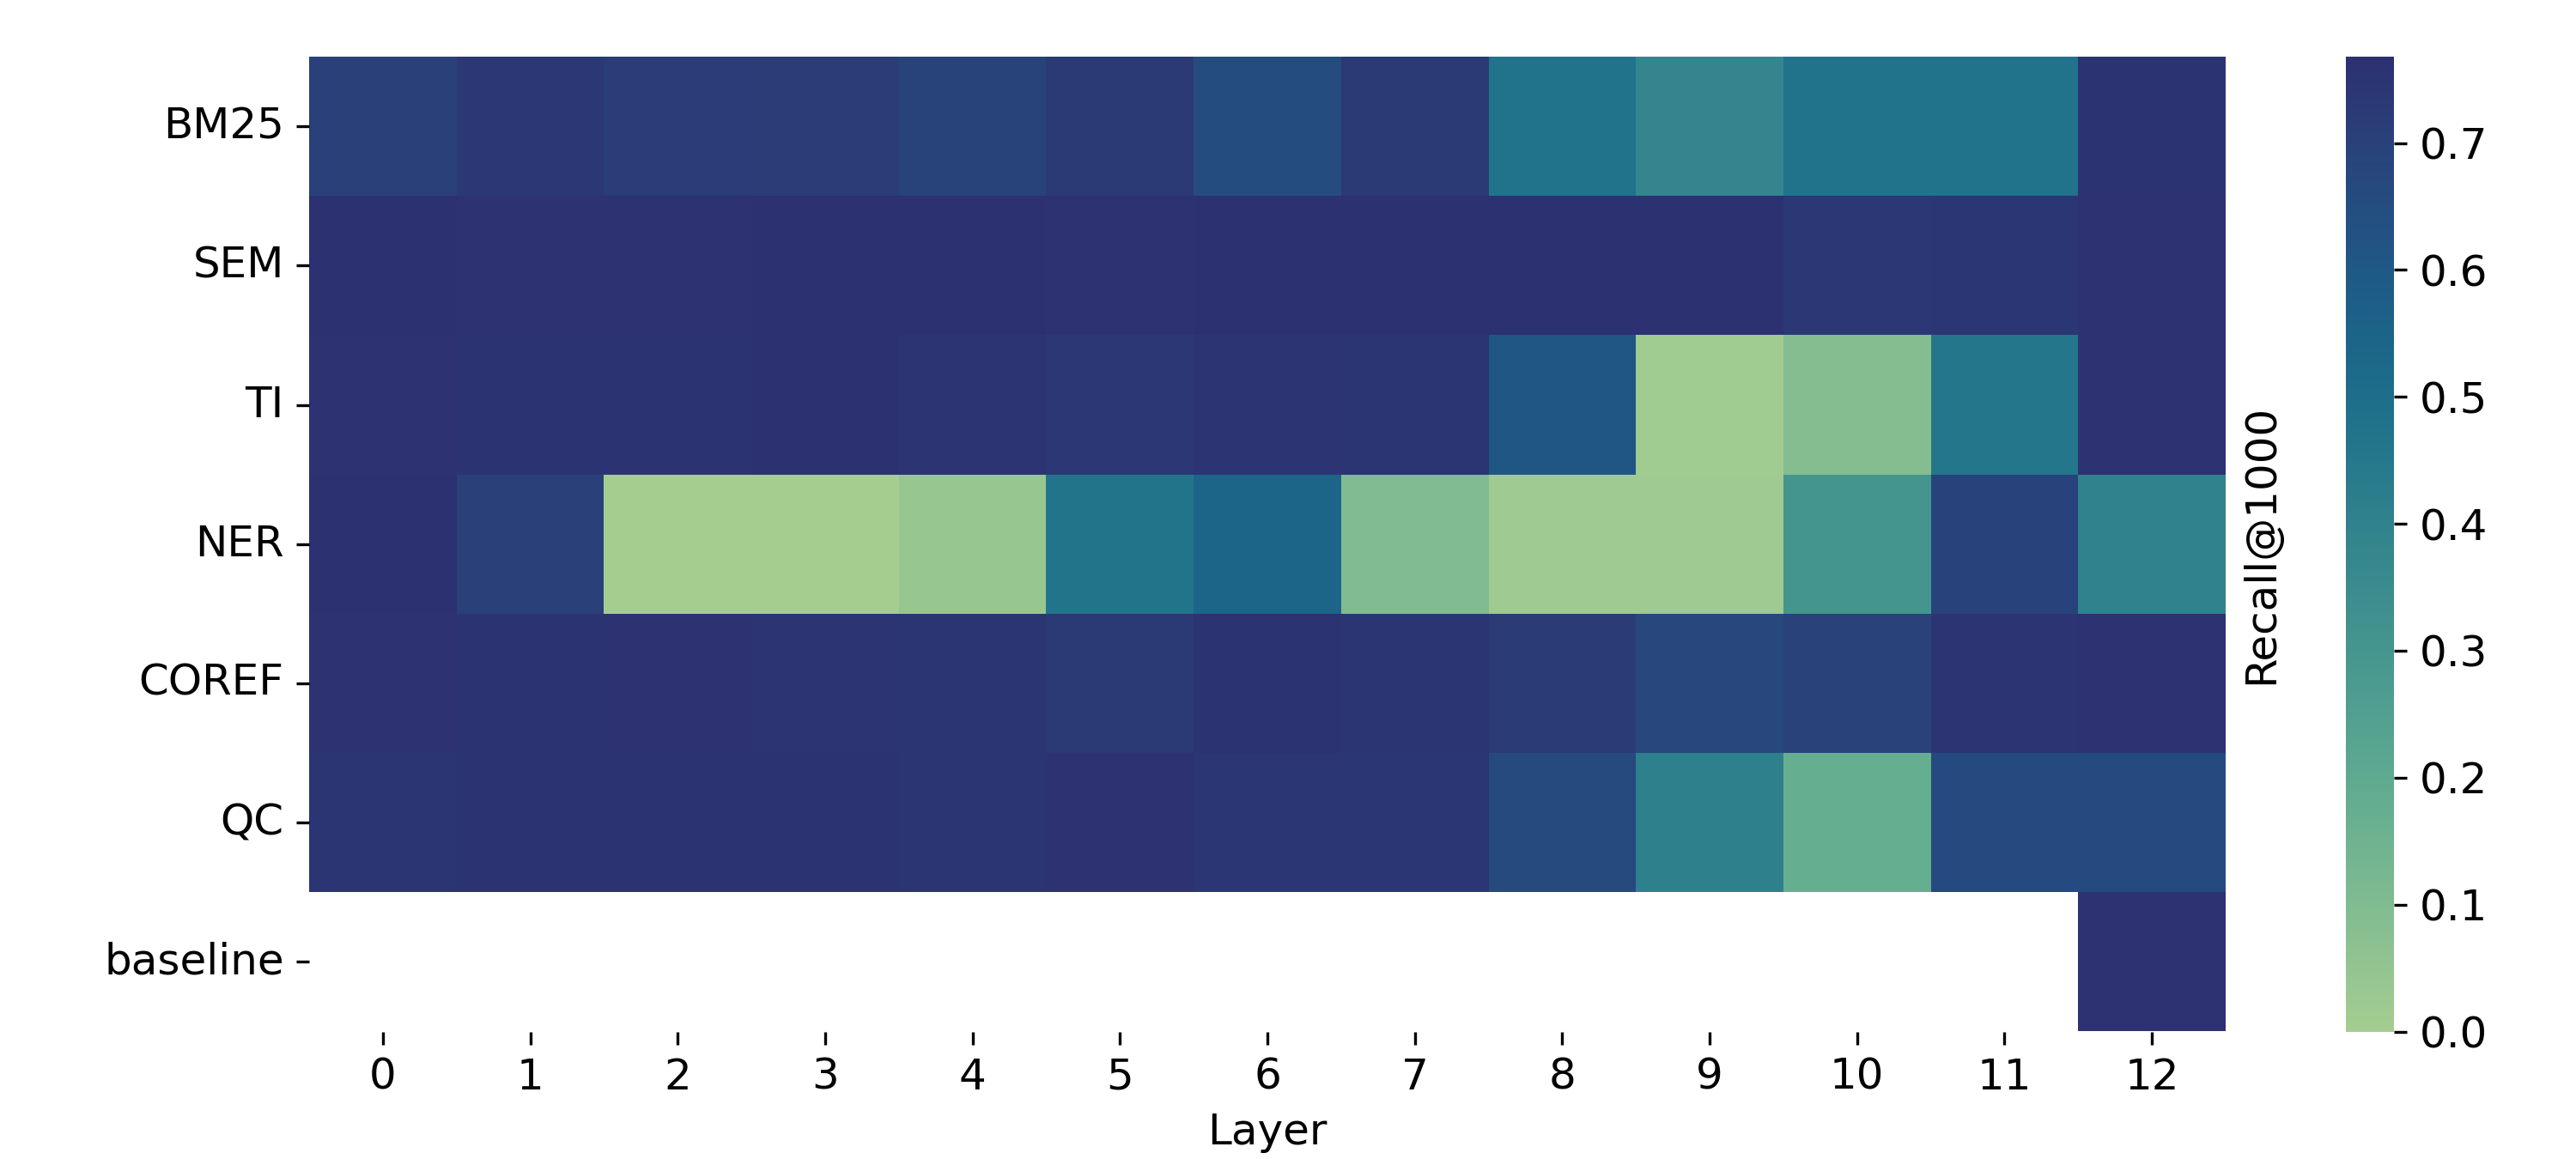
\includegraphics[width=1\textwidth]{figures/all_behaviour_heatmap_recall_1000.png}}
    \end{figure}
\end{frame}

\end{document}